% Chapter 1

\chapter{Litterature Review} % Main chapter title

\label{Chapter2} % For referencing the chapter elsewhere, use \ref{Chapter1} 

%----------------------------------------------------------------------------------------

% Define some commands to keep the formatting separated from the content 


%----------------------------------------------------------------------------------------

\section{Deep Learning-based Semantic Segmentation}\label{soa-sss}

In this section we will discuss different deep learning based segmentation methods. Mostly, a few leading approaches will give an overview of the field.
In Section \ref{seg-in}, an introduction as well as an overview of the research field will be proposed.
Next, in Section \ref{seg1}, we will motivate the choice of these methods by displaying a panel of backbones and networks as well as their respective performances.
Then, in Sections \ref{seg2} and \ref{seg3}, we will learn about methods based on VGG and ResNet respectively, since these are the two most widespread backbones in the domain.
Finally, in Section \ref{seg4}, we will propose a conclusion and a discussion related to the domain.

\subsection{Introduction}\label{seg-in}

Segmentation remain a substantial area of computer vision. It is also historical since it is possible to find contributions proposed in the 70's \cite{ohta1978analysis}. The main idea of the domain is to be able to delimit and differentiate objects/areas. Thus, the segmentation can be assimilated to a transposition of an image space to an intermediate space, semantic or not. That is to say that instead of utilizing colorimetric information, the representation is changed to differentiate the areas of interest.\\

{
\begin{tabular}[h]{p{0.05\textwidth}!{\color{gray}\vrule width 2pt}p{0.7\textwidth}}
	 &\textit{Reminder on semantic with respect to segmentation.}\\
	 &\textit{In addition to partitioning the images, knowledge is infused into the algorithm. For example, a simple threshold is a naive segmentation, segmentation by feature group into several classes can be semantic if the feature space is differentiable and the various labels are identified. }\\
\end{tabular}
}\\


Some multiple approaches can be used to perform a segmentation operation, apart from learning-based ones. Indeed, even before the advent of deep learning, it was possible to divide the domain into five subdivisions: region-based, feature clustering-based, edge-based, threshold-based and model-based.

Region-based and edge-based are two subtypes that are significantly correlated \cite{kaganami2009region,chu1990integration}. It is a question of separating the image using descriptors which have the effect of describing the image using contours from which regions can be deduced. As example, \cite{iannizzotto2000fast, sappa2006unsupervised} both proposed edge-based segmentation and \cite{wani1994edge, mukherjee2014region} proposed contour-based approaches. It is explicit these two techniques are highly linked and seamlessly one can shift to the other and vice versa.


The threshold-based techniques \cite{bhargavi2014survey} are quite naive. Whether the level is deduced iteratively or empyrically, this method consists in fixing a value at which the image will be bounded and then binarized. Predominantly, this technique allows to separate areas like the foreground and background or to highlight recognizable objects.


Conversely, feature-based discrimination can be considered as more advanced or complex. It consists in clustering a group of features that have been previously extracted. This domain has been highly investigated \cite{watt1986feature,li2006new,rashedi2013stochastic}. Indeed, this is likely due to the vast amount of information extractors previously developed. As a consequence, researchers have been able to exploit the acquired knowledge and then derive robust segmentation algorithms.


Finally, model-based segmentation consists in adopting descriptive models to differentiate the objects in the image. Thus, models like the Markov Random Fields Model \cite{marroquin2003hidden}, active shape models \cite{van2002active} and active appearance models have been used to segment images\cite{cootes2001active}.


In spite of all these possibilities and their respective robustness, the algorithms remain rather tied to the applications and unfortunately, they are rather rarely generalizable (viz. when they are designed for one task, they rarely adapt to others).


At present, the vast majority of algorithms have shifted into the field of deep learning. This is purely due to the performance observed with this approach. Thus DL usage allows to prevent the creation of a handmade feature space. In addition, DCNNs have proven their generalization abilities. The primary constraint is the amount of data but once this criterion is met, then the networks have such an abstraction capacity it is unnecessary to explicitly constrain the problem. Hence, some algorithms infuse knowledge into the network even if this practice is quite marginal. Preferably, researchers are seeking blocks or layers that will allow to abstract the data to higher degree and render it more understandable for the algorithms. 


\subsection{Major backbones and network: a comparative evaluation}\label{seg1}

In the semantic learning-based segmentation landscape, a large number of methods are available. Indeed, the field is active and in constant evolution. However, it is possible to extract methods that stand out from the crowd. Moreover, among all the methods, a criterion allows to differentiate them: the backbone.


The backbone represents a term that designates the feature extraction structure. It can also be termed — erroneously — encoder and allows to transpose an image from its initial space to a latent space, usually a feature vector. The concept differentiating the term encoder and backbone is the backbone is predominantly used pre-trained and has been proven for feature extraction and thus classification tasks. On the contrary, an encoder is a general term that only designates an architecture that reduces the dimensionality of the data by densifying the information.

From these feature extractors, a vast number of networks have been derived. Therefore, the models have an already proven part for the classification and extraction task. As a reminder, a segmentation network can be summarized as a classification network with a secondary structure to recover the initial image dimension. It is also possible to call a segmentation network a classification network at pixel level.

To determine the most representative networks and their respective backbone, we propose in Table \ref{tab:segmentationSoA} a quantitative analysis of the results from significant networks on a common benchmark: CityScapes \cite{Cordts2016Cityscapes}. The comparison metrics are Intersections over Union (IoU) by classes or categories initially proposed by \cite{everingham2015pascal}. In addition, the CityScapes benchmark proposed to calculate the iIoU which corresponds to the instance-level IoU and is considered more representative of the actual results\footnote{Calculation of specific metrics and benchmark results available at: \url{https://www.cityscapes-dataset.com/benchmarks/}}.

\renewcommand{\arraystretch}{1.2}
\useunder{\uline}{\ul}{}
\begin{table}[h]
	\centering
	\caption[Overview of major approaches highlighting performances on CityScapes benckmark and backbones.]{Overview of major approaches highlighting performances on CityScapes benckmark \cite{Cordts2016Cityscapes} and backbones. \underline{Underlined} and \textbf{bold} respresents respectively overall second best and best. \textit{Italic} is best per backbone.}
	\label{tab:segmentationSoA}
	\resizebox{\textwidth}{!}{%
		\begin{tabular}{llcllccccc}
			\multicolumn{2}{c}{Backbone} &
			&
			\multicolumn{2}{c}{Approach} &
			&
			\multicolumn{4}{c}{Reported performances on CityScapes Benchmark \cite{Cordts2016Cityscapes}} \\ \cline{1-2} \cline{4-5} \cline{7-10} 
			\multicolumn{1}{l}{Name} &
			\multicolumn{1}{l}{Year} &
			&
			\multicolumn{1}{l}{Name} &
			\multicolumn{1}{l}{Year} &
			&
			IoU class &
			iIoU class &
			IoU category &
			iIoU category \\ \hline
			\multirow{3}{*}{VGG \cite{simonyan2014very}} &
			\multirow{3}{*}{2014} &
			&
			FCN \cite{long2015fully}&
			2015 &
			&
			65.3 &
			41.7 &
			85.7 &
			70.1 \\
			&
			&
			&
			SegNet \cite{DBLP:journals/corr/BadrinarayananH15}&
			2015 &
			&
			57.0 &
			32.0 &
			79.1 &
			61.9 \\
			&
			&
			&
			DilatedNet \cite{yu2015multi} &
			2016 &
			&
			\textit{67.1} &
			\textit{42.0} &
			\textit{86.5} &
			\textit{71.1} \\ \hline
			ReNet \cite{visin2015renet}&
			2015 &
			&
			ReSeg \cite{visin2016reseg}&
			2016 &
			&
			\textit{58.8} &
			\textit{-} &
			\textit{-} &
			\textit{-} \\ \hline
			\multirow{8}{*}{ResNet \cite{he2016deep}} &
			\multirow{8}{*}{2016} &
			&
			PSPNet \cite{zhao2017pyramid}&
			2017 &
			&
			81.2 &
			59.6 &
			91.2 &
			79.2 \\
			&
			&
			&
			RefineNet \cite{lin2016refinenet}&
			2016 &
			&
			73.6 &
			47.2 &
			87.9 &
			70.6 \\
			&
			&
			&
			LKM \cite{peng2017large}&
			2017 &
			&
			76.9 &
			- &
			- &
			- \\
			&
			&
			&
			EncNet \cite{zhang2018context}&
			2018 &
			&
			- &
			- &
			- &
			- \\
			&
			&
			&
			DeepLab v2 \cite{chen2017deeplab}&
			2016 &
			&
			70.4 &
			42.6 &
			86.4 &
			67.7 \\
			&
			&
			\multicolumn{1}{l}{} &
			DeepLab v3 \cite{chen2017rethinking}&
			2017 &
			\multicolumn{1}{l}{} &
			{\ul 81.3} &
			{\ul 62.1} &
			{\ul 91.6} &
			{\ul 81.7} \\
			&
			&
			&
			DeepLab v3+ \cite{chen2018deeplab}&
			2018 &
			&
			\textit{\textbf{82.1}} &
			\textit{\textbf{62.4}} &
			\textit{\textbf{92.0}} &
			\textit{\textbf{81.9}} \\
			&
			&
			&
			Mask-RCNN \cite{he2017mask}&
			2017 &
			&
			- &
			- &
			- &
			- \\ \hline
			\multirow{2}{*}{ResNeXt \cite{xie2017aggregated}} &
			\multirow{2}{*}{2017} &
			&
			DShortcut \cite{bilinski2018dense}&
			2018 &
			&
			- &
			- &
			- &
			- \\
			&
			&
			&
			ExFuse \cite{zhang2018exfuse}&
			2018 &
			&
			- &
			- &
			- &
			- \\ \hline
			MobileNet v1 \cite{howard2017mobilenets}&
			2017 &
			&
			FSTSL \cite{xie2018improving}&
			2018 &
			&
			71.9 &
			- &
			- &
			- \\ \hline
			\multirow{2}{*}{MobileNet v2 \cite{sandler2018mobilenetv2}} &
			\multirow{2}{*}{2018} &
			&
			LWRF \cite{nekrasov2018light}&
			2018 &
			&
			\textit{72.1} &
			\textit{-} &
			\textit{-} &
			\textit{-} \\
			&
			&
			&
			Fast-SCNN \cite{poudel2019fast}&
			2019 &
			&
			68.0 &
			37.9 &
			84.7 &
			63.5 
		\end{tabular}%
	}
\end{table}

This evaluation table shows that mainly two backbones are used, namely VGG and ResNet. This is why the next two sections will be dedicated to these backbones and the networks that operate them.

\subsection{VGG}\label{seg2}

VGG \cite{simonyan2014very}, standing for \emph{Visual Geometry Group}, is an image recognition network that was founded in 2015. It can be considered the pioneer in the field of classification and was, until the appearance of ResNet the only viable backbone.
This encoding network is based on small $3x3$ convolutions and is reasonably simple (compared to recent architectures). Similar to all encoders, it allows to reduce the dimensionality of the input data and to densify it to obtain a representative vector, in particular it encodes an image $MxNx3$ into a feature vector $1x1x1000$. Initially and as shown in Figure \ref{fig:vgg}, $M = 224$ and $N = 224$.

\begin{figure}[h]
	\centering
	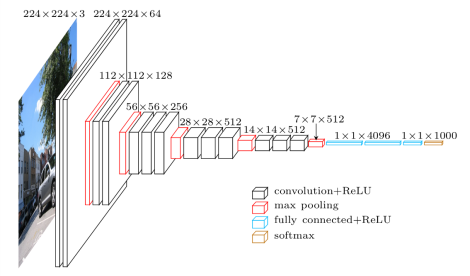
\includegraphics[width=0.5\linewidth]{Figures/SOA/VGG}
	\caption[Simonyan and Zisserman's VGG Architecture.]{Simonyan and Zisserman's \cite{simonyan2014very} VGG Architecture.}
	\label{fig:vgg}
\end{figure}


From its state-of-the-art performances, this network has allowed to derive multiple methods, three of which will be discussed below: FCN \cite{long2015fully}, SegNet \cite{DBLP:journals/corr/BadrinarayananH15} and DilatedNet \cite{yu2015multi}.

\subsubsection{FCN}

\emph{Fully Convolutional Networks} (FCN) \cite{long2015fully}, is an architecture proposed by Jonathan Long, Evan Shelhamer and Trevor Darrell in 2015. It is a highly recognized work to be the "first" pixel-wise semantic segmentation network (PwSS). Wanting to remove the image size constraint, the prevailing idea was to base the architecture solely on convolution layers. Convolution effectively represents a valid technique ensuring the same image size at the output of the pipeline. 
However, the challenge was predominantly based on this dimensionality. As follows, Long et al. proposed an approach based on pooling and deconvolution to retrieve the image dimension while keeping the semantic segmentation information across layers.
While the encoder extracts the information and interprets the image, the decoder considers the task of increasing the dimension while keeping the localization aspect. Only, the effect of downsampling allows reducing the dimension but at the cost of the resolution and the definition when proceeding to the upsampling. In response to this phenomenon, Long et al. introduced the concept of skip connection allowing an aggregation, in the decoder, of information coming directly from the encoder. By this approach, the model is efficient to infer fine-grained segmentation while taking advantage of the dimensionality reduction of the encoder.


\subsubsection{SegNet}

SegNet \cite{DBLP:journals/corr/BadrinarayananH15} is a network highly inspired by FCN but uses other innovative principles. While Long et al. proposed the skip connection concept, SegNet proposes a symmetric architecture with VGG.
And, as a replacement to skip connections, Badrinarayanan et al. develop the principle of indexed pooling. The encoder uses maxpooling operations to reduce the dimension and obtain a feature vector. From this pooling block, an information map of lower dimensionality and an index map is extracted. This index map will then be used in the unpooling operations of the decoder to "reconstruct" the segmentation map with a proper positioning. 



\subsubsection{DilatedNet}

In this approach Yu et al. \cite{yu2015multi}, instead of attempting sampling-based approaches, investigated the concept of dilated convolution. Thus, DilateNet is illustrated by its structure using the dilation properties of convolutions to reduce or increase the size of the maps. The idea is based on this concept of densification of feature maps but also on the increase of the range (i.e. the receptive field) of the convolutions. The advantage is that, for the same impact on the images, the use of dilation allows a much lesser use of parameters and thus the complexity of the networks is decreased by this way. As stated by the authors : \emph{"the receptive field grows exponentially while the number of parameters grows linearly"}.


\subsection{ResNet}\label{seg3}

ResNet \cite{he2016deep} is another backbone and it can undoubtedly be considered as the most widespread in all domains including deep learning based models. The creation of this architecture starts from an observation. Prior to this contribution, the community assumed that the deeper the network, the better it performed. This is legitimate and verifiable, but it is straightforward to observe that in reality, after a certain number of layers, the network loses resolution and performance. This fact comes from a recurrent problem in the learning task: the \emph{vanishing gradient}. After an certain amount of operation, the results are largely approximated by the standard algorithmic methods such as rounding or floating point precision. This would suffer no impact if the training did not require back propagation. Thus, during the propagation, due to the approximation, the floating point estimate \cite{gysel2016hardware} or simply the chain rule \cite{leibniz} used during the calculation of the gradient, the loss shrinks to zero. This vanishing gradient problem prevents the layers from updating and the network does not train anymore.

\begin{figure}[h]
	\centering
	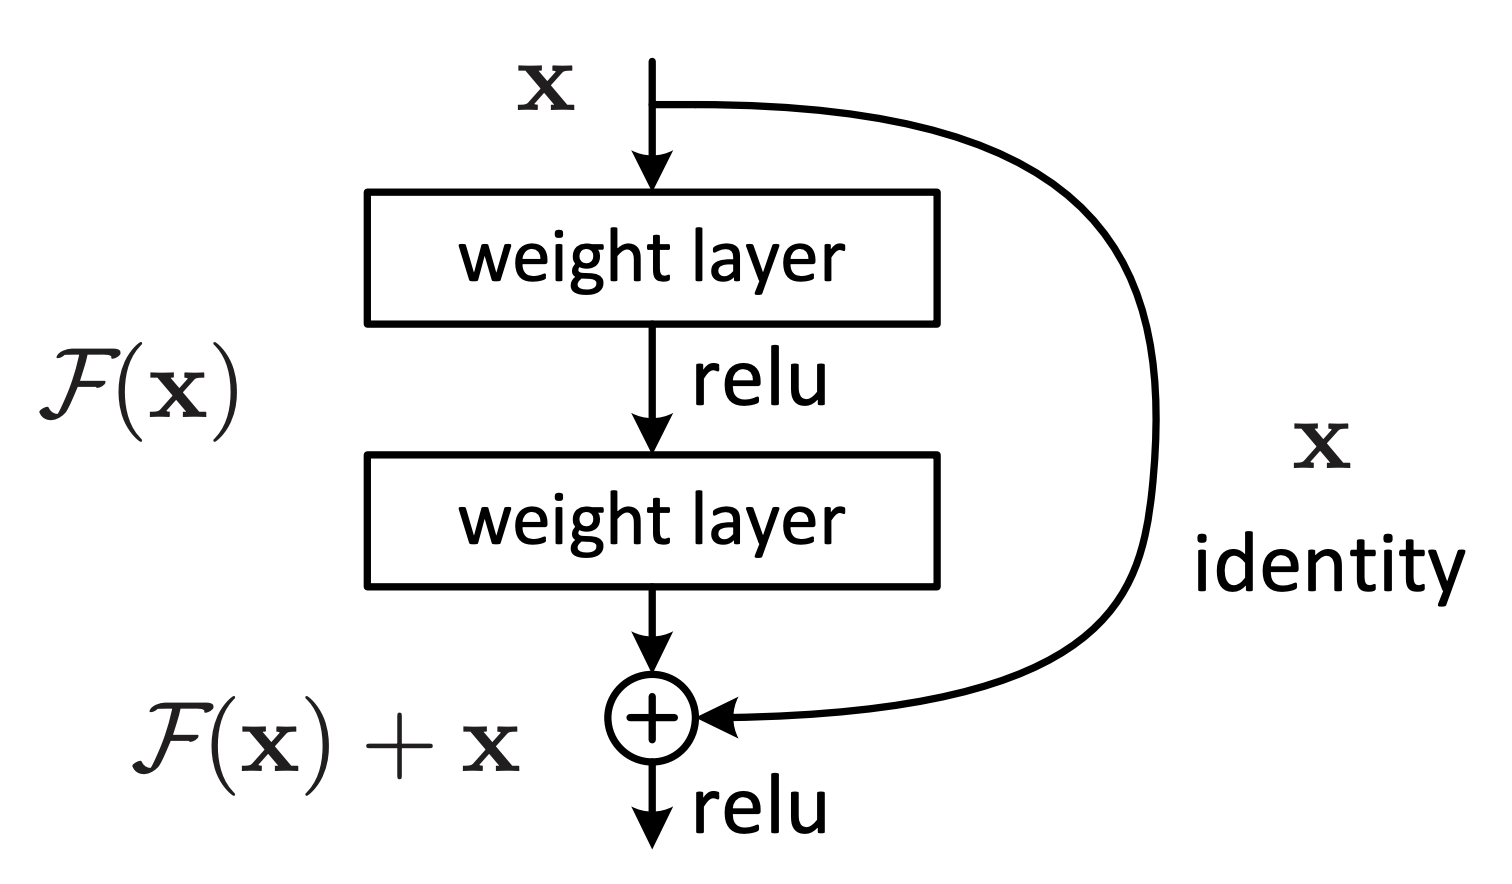
\includegraphics[width=0.6\linewidth]{Figures/SOA/resnetblock}
	\caption[Illustration of ResNet block.]{Illustration of ResNet \cite{he2016deep} block.}
	\label{fig:resnetblock}
\end{figure}


ResNet overcomes this problem by implementing layer-wise skip connections that allow the gradient to be transmitted smoothly (shown in Figure \ref{fig:resnetblock}). By adopting this strategy, it is then possible to use the starting postulate and increase the size of the networks. Once the vanishing gradient is eliminated, nothing prevents the densification of the networks since the skip connections allow the transmission of information.

\subsubsection{PSPNET}

\emph{Pyramid Scene Parsing Network} (PSPNet) \cite{zhao2017pyramid} is a pixel-wise semantic segmentation network derived from ResNet classifiction network. 
This contribution is focused on an innovative sampling method based on a multi-layer pyramid. The approach called \emph{pyramid pooling} is an architecture in four levels (instead of one traditionally). Considered to keep the context of the images, the four stages of the pyramid consider in parallel the whole, half or portions of the base image. Ultimately, whether it is the first feature extraction or the output of each layer of the pooling structure, all this information is adapted in dimensions and concatenated. All this followed by a dense convolution allows keeping both the local and global context of the image and thus to maintain the information across layers. Thus, the loss of information is reduced which allows to have sharp edges and accurate estimations of the classes according to the features extracted by the numerous layers of the network.

\subsubsection{DeepLab}

There are multiple versions of DeepLab. However, it is possible to summarize the ResNet-based contributions into some key concepts brought by Chen et al. \cite{chen2018deeplab}.
First, the global architecture is based on dilated convolutions or atrous convolutions. As expressed for DilatedNet, this operation allows many advantages like dimensionality reduction or judicious management of the receptive field.

Subsequently, this method proposes the use of bilinear interpolation which seems to represent a naive approach to upsampling. In practice, the authors expressed the use of another dimensionality recover strategy is not especially necessary to obtain efficient results.

Ultimately, the contribution proposes the use of \emph{fully connected CRF}. The principle is to consider the pixels as a node in a graph and that all these nodes are connected by different means. Thus, the idea is to enforce the assignment of similar labels to adjacent pixels. The usefulness of this kind of structure could be justified by the classification of areas instead of dependent pixels. Thus, this architecture allows to keep a coherent structure and reduce the aberrations of segmentations with nested classes. In addition, fcCRFs shows great performances with regard to the edges and the object separation.
The contribution of the CRF conveys enormous complexity to the network, but some demonstrations \cite{krahenbuhl2011efficient} has made it possible to remove certain constraints and thus make this type of structure viable.
It is nevertheless considerable this brings a great number of additional parameters and especially increases the complexity of the networks.
To conclude on this architecture that is DeepLab, it remains to this day (with its declensions) the state-of-the-art method for segmentation. Some networks highlight better class-wise performances but include a cost and a disproportionate complexity compared to the difference in efficiency.

\subsection{Conclusion and discussion}\label{seg4}

After briefly explaining the major backbones and their main derived segmentation architecture, it was illustrated that learning-based segmentation has been a flagship field in computer vision. The recorded performances presented in the comparative study are far superior to observations prior to the advent of deep learning. However, it is possible to see this field is almost at the end of its course since the performances tend to stagnate and the research to move towards other processes of understanding. The emergence of instance segmentation or geometric understanding of scenes tends to reduce the amount of contribution in PwSS.

Despite this observation, it is also quite possible to note the algorithms are subject to the same constraints as any deep learning algorithm, namely the need for data. Plus, an overwhelming majority classify colorimetric images and assume these data are thoroughly characteristic of the observed scenes. There is a considerable knowledge in the field of segmentation, but it has rarely been exported to other types of data to see if the performance on similar tasks can be improved by a strategic use of the data.
Hence, the answer might not be to depend on the depth and number of layers of the network but to shift the data space to something more characteristic. 
%----------------------------------------------------------------------------------------
\pagebreak
\section{Depth Estimation}\label{soa-de}

In this section of the literature review, various concepts related to depth will be discussed. Starting from the principal acquisition technology in part \ref{depth-acqu}, we will continue on the learning-less methods for depth estimation in part \ref{multi-im}.
Ultimately, we will more deeply discuss the concept of learning-based depth estimation from a monocular in part \ref{mono-im} since this is the topic on which part of this manuscript is devoted.


\subsection{Laser-based imaging}\label{depth-acqu}

Laser-based imaging is a frequently used method for its accuracy and robustness. Indeed, it allows, regardless of the conditions of illumination or distance, to accurately estimate the distance sensor-object using a laser projection.
There is a wide variety of different sensors, and their performance is highly correlated with their price. Indeed, while some devices allow a smooth acquisition of several thousand points or at distances of several hundred meters, others are relatively limited in capacity. Despite this, the overall acquisition principle remains the same and is uninfluenced by this disparity in performance.
The concept is considerably classic, a laser is projected on a surface that will then reflect it. As follows, it is possible to calculate the distance by measuring the time elapsed between the emission and reception. 
However, the whole principle is based on reflection. As a result, this approach can be inefficient especially when the target scenes include specular surfaces \cite{hrabar2012evaluation} (e.g. mirrors, glass, water, and other reflective surfaces).
It also turns out these sensors can be made deficient in adverse weather conditions. In particular when the projected laser can be refracted in rainy weather or altered in foggy weather.
Conversely, few approaches are as robust in favorable meteorological circumstances. Therefore, most datasets containing target depth maps use laser-based imaging like KITTI\cite{Geiger2012CVPR,Menze2015CVPR,Fritsch2013ITSC} and its LiDaR setup. But, the data contain a bias since they were acquired mainly in favorable conditions.

\begin{figure}[h]
	\centering
	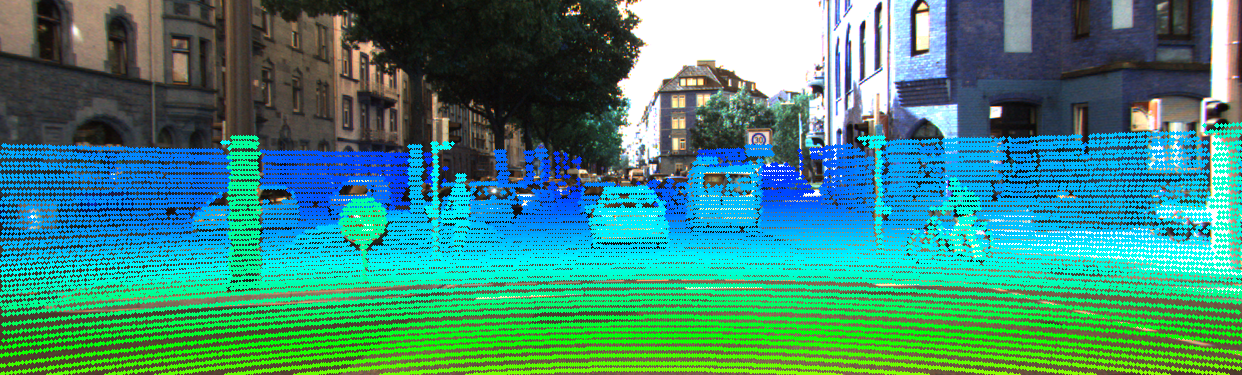
\includegraphics[width=0.8\linewidth]{Figures/SOA/lidar-ill}
	\caption[Illustration of LiDar point-cloud.]{Illustration of LiDar point-cloud\footnotemark. Sparsity can be observed as well as erroneous estimation on vehicle windows.}
	\label{lidar-ill}
\end{figure}



The LiDar, \emph{laser imaging, detection, and ranging}, is a laser rangefinder commonly used since it is motorized and rotatable \cite{wang20133d}. Rotating at 360$^\circ$ at a considerable speed, it allows to make panoramic acquisitions. Moreover, LiDaR are classified according to their number of slices, which gives them, not only a horizontal but also a vertical acquisition. Thus, the more slices, the more vertical points are acquired "semi-simultaneously".
As shown in Figure\ref{lidar-ill}\footnotetext{Image borrowed from \url{henryzh47.github.io}}, the generated point cloud can be affixed to the colorimetric image corresponding to the scene. This illustration also highlights the defects related to specular surfaces, here, the vehicle windows.

In spite of this considerable estimation power, it should be noted that this operation contains flaws of which two critical ones are identifiable. The acquisition of moving objects, especially if the relative speed between sensor and target is high, can be very inaccurate. The second drawback comes directly from the acquisition technology. A multitude of points is projected in the surrounding space. As previously discussed, even if it depends on the size of the pattern, only points are acquired \cite{vaze2007high}. As a consequence, the deduced point clouds are very sparse, and this factor is aggravated by the distance between an object and the sensor (visible in Figure\ref{lidar-ill}). As a result, the depth maps are sparse or subject to interpolation to fill this sparsity.

In conclusion, LiDaR remain a robust tool for scene depth estimation. Regrettably, this device can be expensive or inefficient. As a result, the Computer Vision community tends to find estimation algorithms at the expense of this scanner and its drawbacks.

\subsection{Multi-image methods}\label{multi-im}

Multi-image based depth estimation methods have been developed for several purposes. One of the main ones is the access to this kind of technique since it does not require a complex acquisition system. Indeed, standard cameras can be used to recover the depth. 

These algorithms can be separated in two main parts: Multiple camera systems described in part \ref{mcs}, and Single camera systems in part \ref{scs}.

\subsubsection{Multiple camera systems}\label{mcs}
One of the best-known approaches in the field of multi-camera systems is stereovision. Highly inspired by human biology\cite{marr1979computational}, this technique consists in the use of two cameras similarly to the eyes.

From this acquisition system, two different points of view are obtained and then allow the matching of points of interest. The concept is based on the transposition of points from a three-dimensional space to a two-dimensional image plane.
Hence, starting from a 3D point with homogeneous coordinates, it is possible to transpose it into the image frame such that:

\begin{equation}
	\begin{pmatrix}
	x \\ y \\ 1
	\end{pmatrix} = kP \begin{pmatrix}
	X \\ Y \\ Z \\ 1
	\end{pmatrix},
\end{equation}

with $(x,y,1)^T$ the 2D coordinates and $(X,Y,Z,1)^T$ the 3D coordinates with both ones the scale parameter of the point. Plus, $k$ represents the scale factor and $P$ the projection matrix.

$P$ is a constraining matrix that contains the intrinsic parameters of the camera and the extrinsic parameters. 
These two parameters are respectively the proper properties of the camera independent of any external factor, and the information necessary for the positioning of the camera in the world frame like a $3x3$ rotation matrix and a $3x1$ translation vector.
To find these two parameters, P is decomposed as follows:

\begin{equation}
	P = \underbrace{\begin{pmatrix}
	f_x & 0 & x_0 \\
	0 & f_y & y_0 \\
	0 & 0 & 1
	\end{pmatrix}}_K \underbrace{\begin{pmatrix}
	R_{00} & R_{01} & R_{02} & t_x \\
	R_{10} & R_{11} & R_{12} & t_y \\
	R_{20} & R_{21} & R_{22} & t_z \\
	0 & 0 & 0 & 1
	\end{pmatrix}}_E.
\end{equation}

In this manner, it is possible to retrieve the intrinsic parameters matrix $K$ composed of: $f_x$ and $f_y$ the oriented focal distance in the image, and ($x_0$,$y_0$) the centroptic coordinates in the image frame. In addition, we can recover the rotation matrix $R$ as well as the translation vecotr $t$ with respect to the world frame in the extrinsic parameters matrix $E$. Note, the constraining aspect of $P$ comes from the necessity of these parametric matrices $\{K,E\}$ since this implies a calibration of the system.

\begin{figure}[h]
	\centering
	\begin{subfigure}{.8\textwidth}
		\centering
		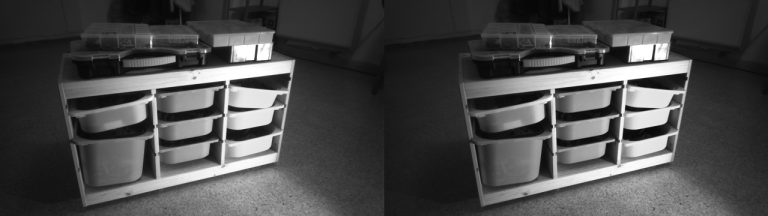
\includegraphics[width=\linewidth]{Figures/SOA/rectified-768x216}
	\end{subfigure}
	\begin{subfigure}{.8\textwidth}
		
		\centering
		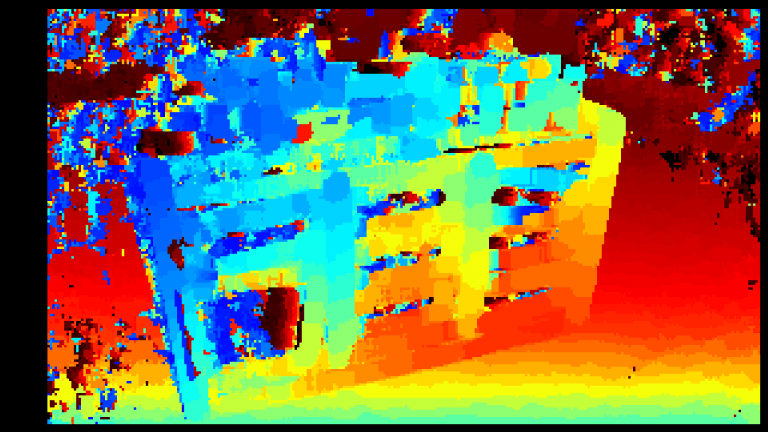
\includegraphics[width=\linewidth]{Figures/SOA/ssd-depth-768x432.png}
	\end{subfigure}
	\caption[Intel RealSense acquisition and reconstruction example.]{Intel RealSense acquisition and reconstruction example. Top row is the rectified images from the camera, bottom row is the obtained reconstruction.}
	\label{intel}
\end{figure}

Conversely, as soon as the sine qua non camera calibration condition is verified, these equations are solvable. This allows us to find the coordinates of 3D points as long as we can identify them in the two or $N$ views. Hence, whether the system is binocular in stereovision as shown in Figure \ref{intel}, or whether the cameras are multiplied in a multi-view system, the problem is reduced to the matching of points identifiable through different views.
As proves \cite{bensrhair1996fast,banks2001quantitative,scharstein2002taxonomy,gehrig2009real} for stereovision, or \cite{hartley1994projective,hartley2000zisserman,campbell2008using} for multiple view reconstruction, this domain has been thoroughly investigated.
Over the years, the research community oriented these approaches towards the real time / online estimation through FPGA embedding \cite{banz2010real}, optimization improvements \cite{kolmogorov2002multi, michael2013real,rodriguez2017improve} or even speed enhancements \cite{feng2019asv}.

Since the system is identified from the stage where it is calibrated, and thus the problem relies almost solely on matching, then many feature differentiation methods have emerged to advance the field.


Thus, different information extraction approaches such as: brightness-based \cite{gennert1988brightness}, segment-based \cite{sumi20023d}, feature-based \cite{se2001vision} or segmentation-based \cite{bleyer2004layered}, have contributed to the progress of multi-image reconstruction.

\begin{figure}[h]
	\centering
	\begin{subfigure}{.3\textwidth}
		\centering
		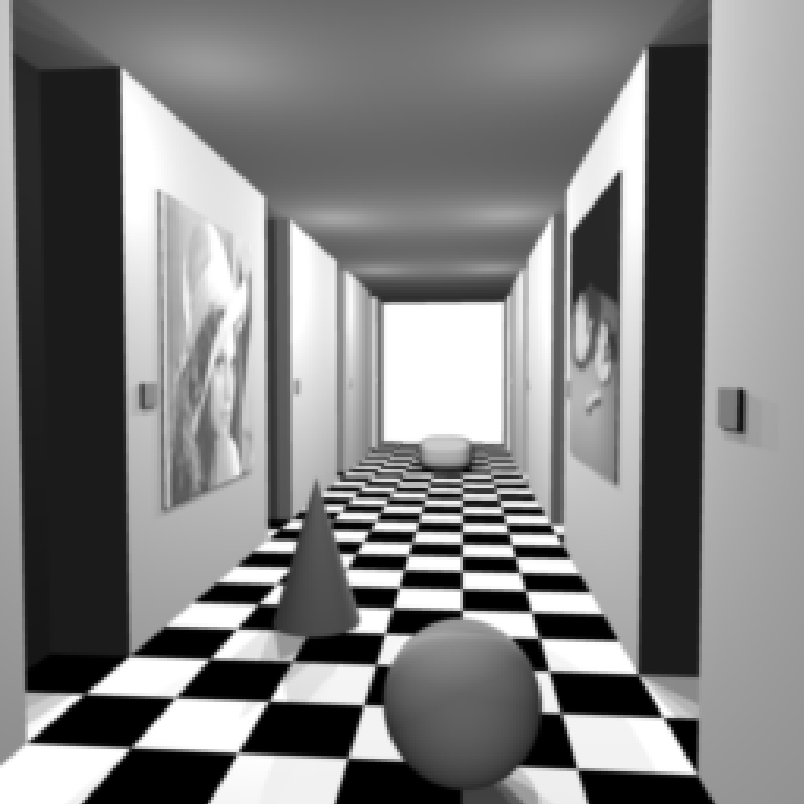
\includegraphics[width=\linewidth]{Figures/SOA/wood1.png}
	\end{subfigure}
	\begin{subfigure}{.3\textwidth}
		
		\centering
		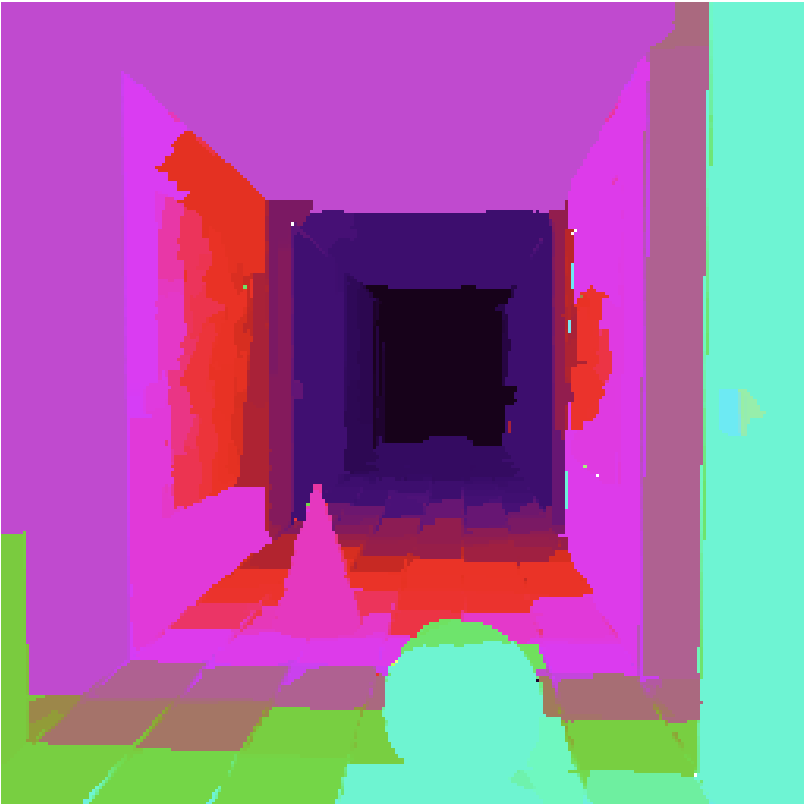
\includegraphics[width=\linewidth]{Figures/SOA/wood2.png}
	\end{subfigure}
	\begin{subfigure}{.3\textwidth}
		
		\centering
		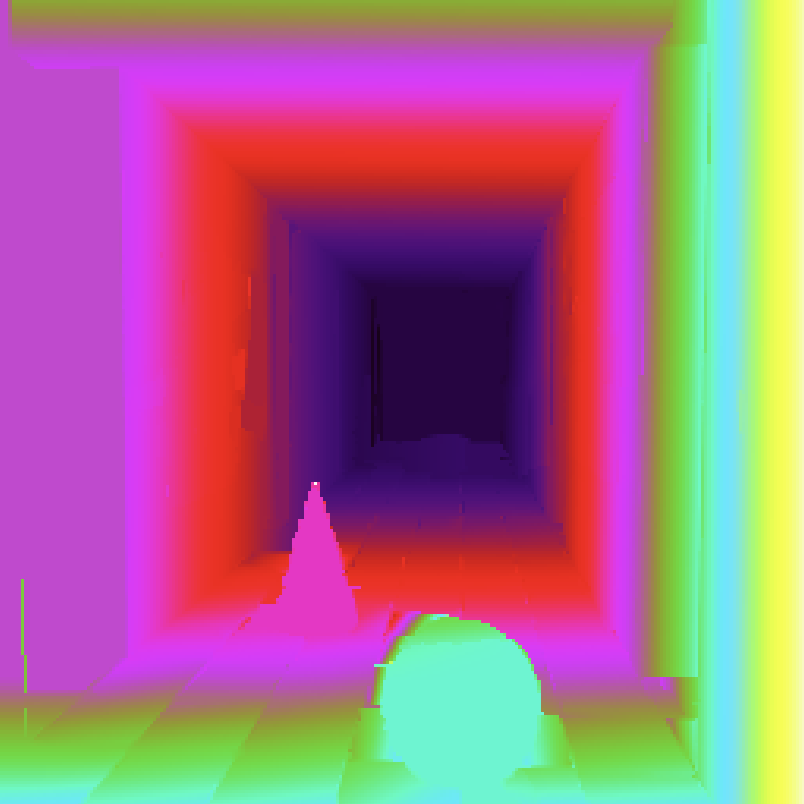
\includegraphics[width=\linewidth]{Figures/SOA/wood3.png}
	\end{subfigure}
	\caption[Illustration of stereovision depth estimation using Woordfor et al. method.]{Illustration of stereovision depth estimation using \cite{Woodford2008GlobalPriors} method. From left to right: reference image, first order reconstruction and second order reconstruction.}
	\label{illu-wood}
\end{figure}

However, to deepen only one contribution, Woordford et al. \cite{Woodford2008GlobalPriors} proposed new optimization approaches leading to leveraging graph cuts to relief surface-orientation major constraint. Therefore, while previous algorithms were struggling while addressing non-fronto-parallel surfaces, they succeeded into integrating second order derivatives leading to more accurate and reliable depth maps. Thus, this method allowed smoother and more precise surface reconstruction in realistic conditions. As shown in Figure \ref{illu-wood}, depth estimation became finer as \cite{Woodford2008GlobalPriors} has been used.

Despite of all the numerous contributions on the multi-image concept and the considerable reconstructions accuracy, still some significant drawbacks subsist. First, as it was discussed above, the calibration aspect represents a key constraint for the acquisition system as well as its deployability. Secondly, as it was highlighted, even if a considerable amount of approaches focuses on features recognition, stereo matching by definition requires features. Unfortunately, the acquisition may observe textureless areas which leads to unsolvable problem. 
Last, the acquisition system requires two or more cameras, and this by essence could be problematic. In response, some methods lift this last constraint by operating a single camera.

\subsubsection{Single camera systems}\label{scs}

Depth estimation from a unique image prevents material constraints but raises other questions. Indeed, the use of such a setup prevents the use of triangulation made possible by the use of multiple sensors.
Therefore, innovative approaches named Shape-from-X (SfX) have emerged. In this framework, X represents several possible cues like motion\cite{caine1993design,dellaert2000structure,chhatkuli2014non,parashar2016isometric}, shading\cite{horn1986variational,zhang1999shape}, blur\cite{favaro2005geometric,zhuo2009recovery}, texture variation \cite{aloimonos1988shape} etc.

As a deepened example, Favaro and Soatto \cite{favaro2005geometric} proposed a original approach to benefit from de-focus phenomenon. 

\begin{figure}[h]
	\centering
	\begin{subfigure}{.3\textwidth}
		\centering
		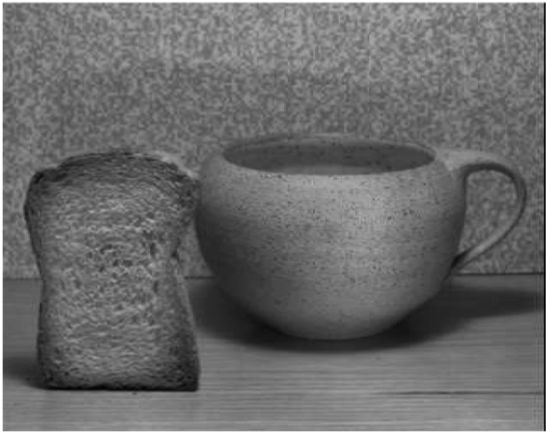
\includegraphics[width=\linewidth]{Figures/SOA/fav1.png}
	\end{subfigure}
	\begin{subfigure}{.3\textwidth}
		
		\centering
		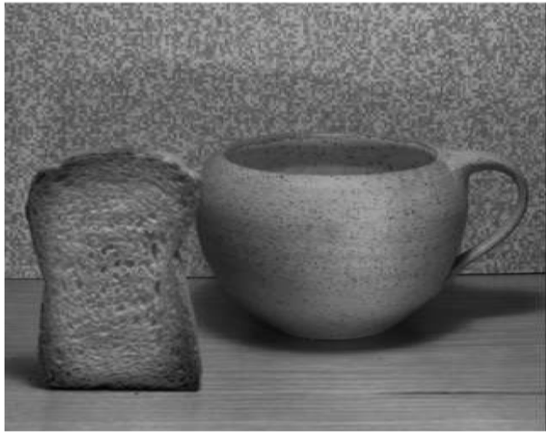
\includegraphics[width=\linewidth]{Figures/SOA/fav2.png}
	\end{subfigure}
	\begin{subfigure}{.3\textwidth}
		
		\centering
		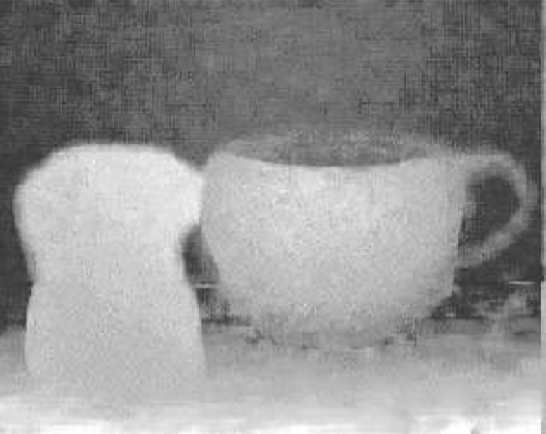
\includegraphics[width=\linewidth]{Figures/SOA/fav-r.png}
	\end{subfigure}
	\caption[Estimate computed from Favaro and Soatto's method.]{Estimate computed from Favaro and Soatto's method \cite{favaro2005geometric}. The two left images shows different images from the focus point of view. The right image display the result of their reconstruction approach.}
	\label{illufavaro}
\end{figure}

The proposition is such that from two images with different camera settings, implying dissimilar focus, they propose computing either:

\begin{itemize}
\item an optimized inference when \emph{point spread function} (PSF) \cite{rossmann1969point} is known
\item kernelized orthogonal operator through convolution
\end{itemize}

to estimate the 3D geometry of the scene. As shown in Figure \ref{illufavaro}, with two acquisition of a scene with different focus (two left images), a depth can be infered (right image) just by a blur-focused algorithm.


\begin{figure}[h]
	\centering
	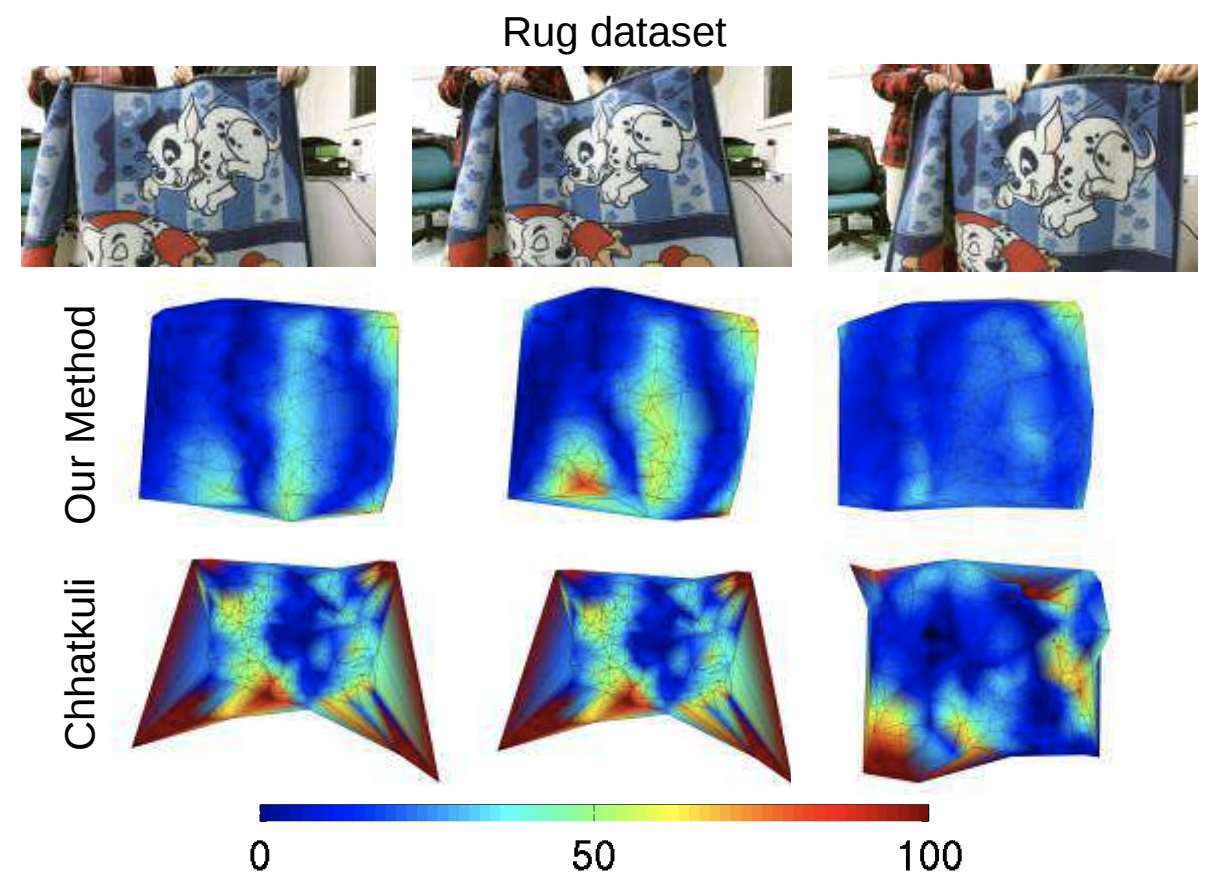
\includegraphics[width=0.8\linewidth]{Figures/SOA/parshar}
	\caption[Example of estimates from Parashar et al.]{Example of estimates from Parashar et al.\cite{parashar2016isometric}. From top to bottom are: input images with deformable object wrapped over time, reconstruction error from \cite{parashar2016isometric} and reconstruction error from \cite{chhatkuli2014non}.}
	\label{illuparshar}
\end{figure}


More recently, Parashar et al. \cite{parashar2016isometric} contributed in the field of shape-from-motion. They propose addressing \emph{Isometric Non-Rigid Shape-from-Motion} which consists of reconstructing a non-rigid object observing shape variation over time. To accomplish such a task, they introduce Riemmanian manifolds-based\cite{lee2006riemannian} representation of the deformable 3D surface. To such a degree, they succeed into modelizing the warps applied to the non-rigid object over time. As shown in Figure \ref{illuparshar}, the proposed method showed increased performances compared to \cite{chhatkuli2014non}.


Despite all these advanced methods, it is considerable that the computational complexity of such algorithms is extremely high. As the sophistication of the algorithms increases, the performance and usability suffer.



In conclusion, despite the fact that the problem of single-camera depth estimation generates an infinite number of solutions and therefore the problem is considered to be ill-posed, the scientific community has been able to adopt innovative approaches to resolve the difficulties. Thus, at the cost of this increased complexity, the acquisition systems could be lightened and SfX field has proposed modern alternatives for depth estimation.
However, the arrival of learning with the growth of computational power has allowed the development of learning-based approaches. 

\subsection{Learning-based monocular depth estimation}\label{mono-im}

In the previous section, we saw it was possible, from several images, whether from one or more cameras, to estimate a depth map. However, each method based on "standard image processing" contains considerable drawbacks. 
With the advent of Deep Learning, many codes has been turned upside down and depth estimation is no exception. Indeed, in essence, learning should relax the constraints by taking advantage of a massive amount of computation. 

These learning-based methods can be divided into two distinct parts, (semi-)supervised learning and self-supervised learning, which will be explained in parts \ref{ssl} and \ref{usl} respectively.

\subsubsection{(Semi-)supervised learning}\label{ssl}

This deep learning process\footnote{Here, the choice was made not to dissociate semi-supervised and supervised learning since they are based on the equivalent concept.} is excessively used as seen in section \ref{soa-sss}, and as for segmentation, for depth estimation, it requires a considerable amount of annotated data. Indeed, as segmentation requires label maps, DCNN-based depth estimation requires reference depth maps.

The problem is thus formulated differently. While previous methods required a characterization of the essential information to match across views, learning-based methods learn by themselves the necessary feature space, provided they utilize a consistent and representative amount of data.

Among the first to investigate the benefit of a profusion of aligned RGB-D data, Eigen et al.\cite{eigen2014depth} were able in 2014 to show that despite an ill-posed problem (as expressed in \ref{scs}), it is possible to obtain sustainable results.

\begin{figure}[h]
	\centering
	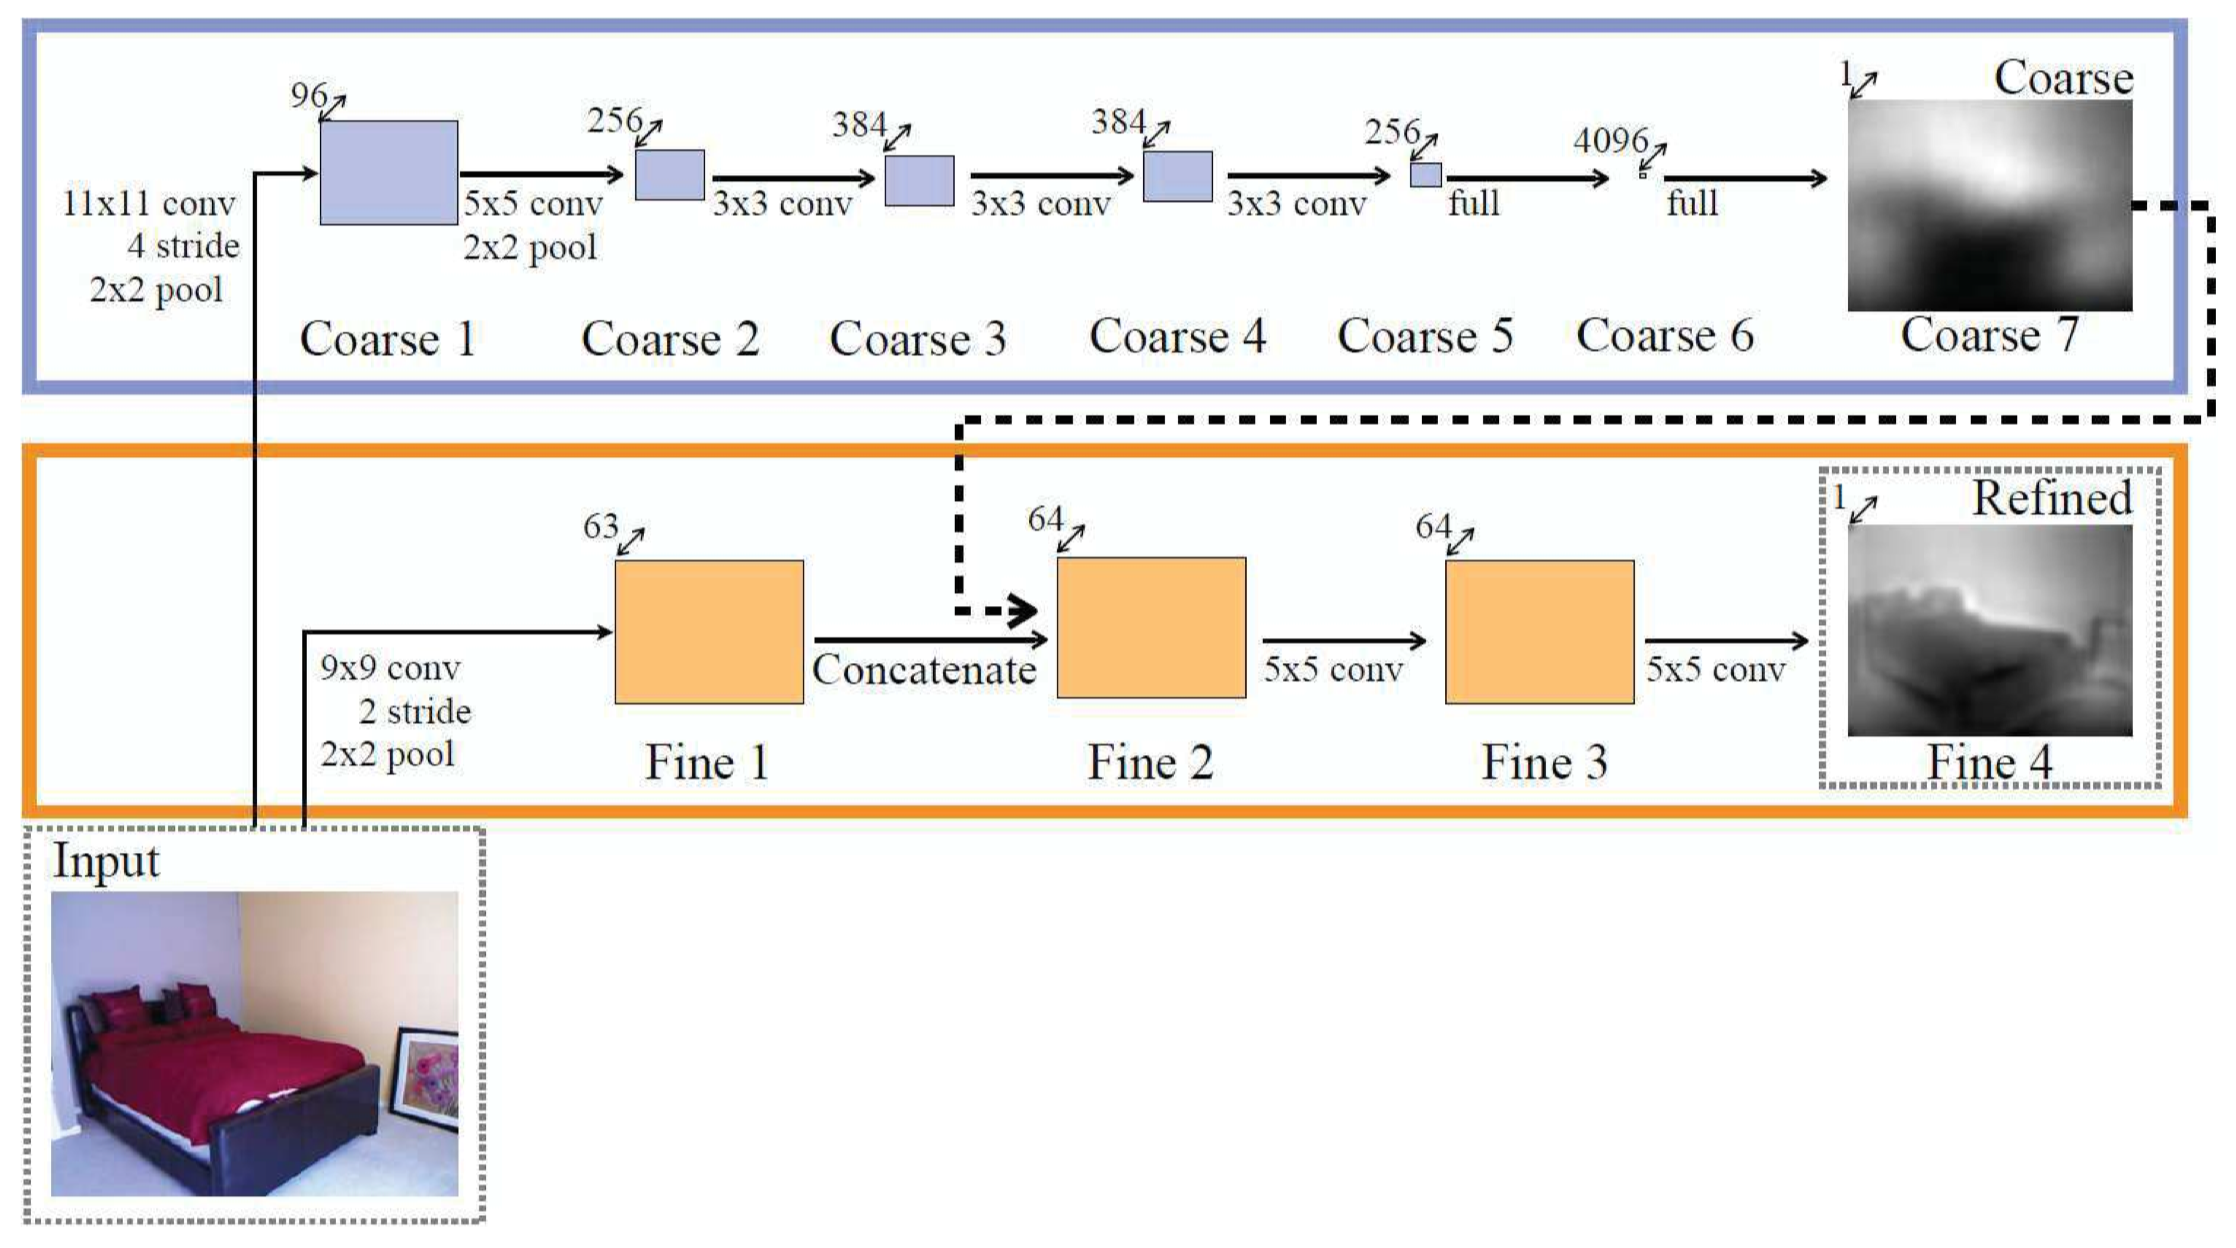
\includegraphics[width=0.8\linewidth]{Figures/SOA/arch-eigen}
	\caption[Eigen et al. Architecture.]{Eigen et al.\cite{eigen2014depth} Architecture.}
	\label{arch-eigen}
\end{figure}


By implementing a biphasic network (shown in Figure \ref{arch-eigen}) allowing the estimation of two depth maps, one coarse and the other refined, while proposing the use of a scale-invariant loss, they were capable to take advantage of rich annotated data sets such as NYU \cite{SilbermanECCV12} and KITTI \cite{Geiger2012CVPR,Fritsch2013ITSC,Menze2015CVPR}.
The contribution is twofold, firstly the cascade network of which the first one, from which the coarse map results, is not completely convolutional (last two layers dense and fully connected). 


\begin{figure}[h]
	\centering
	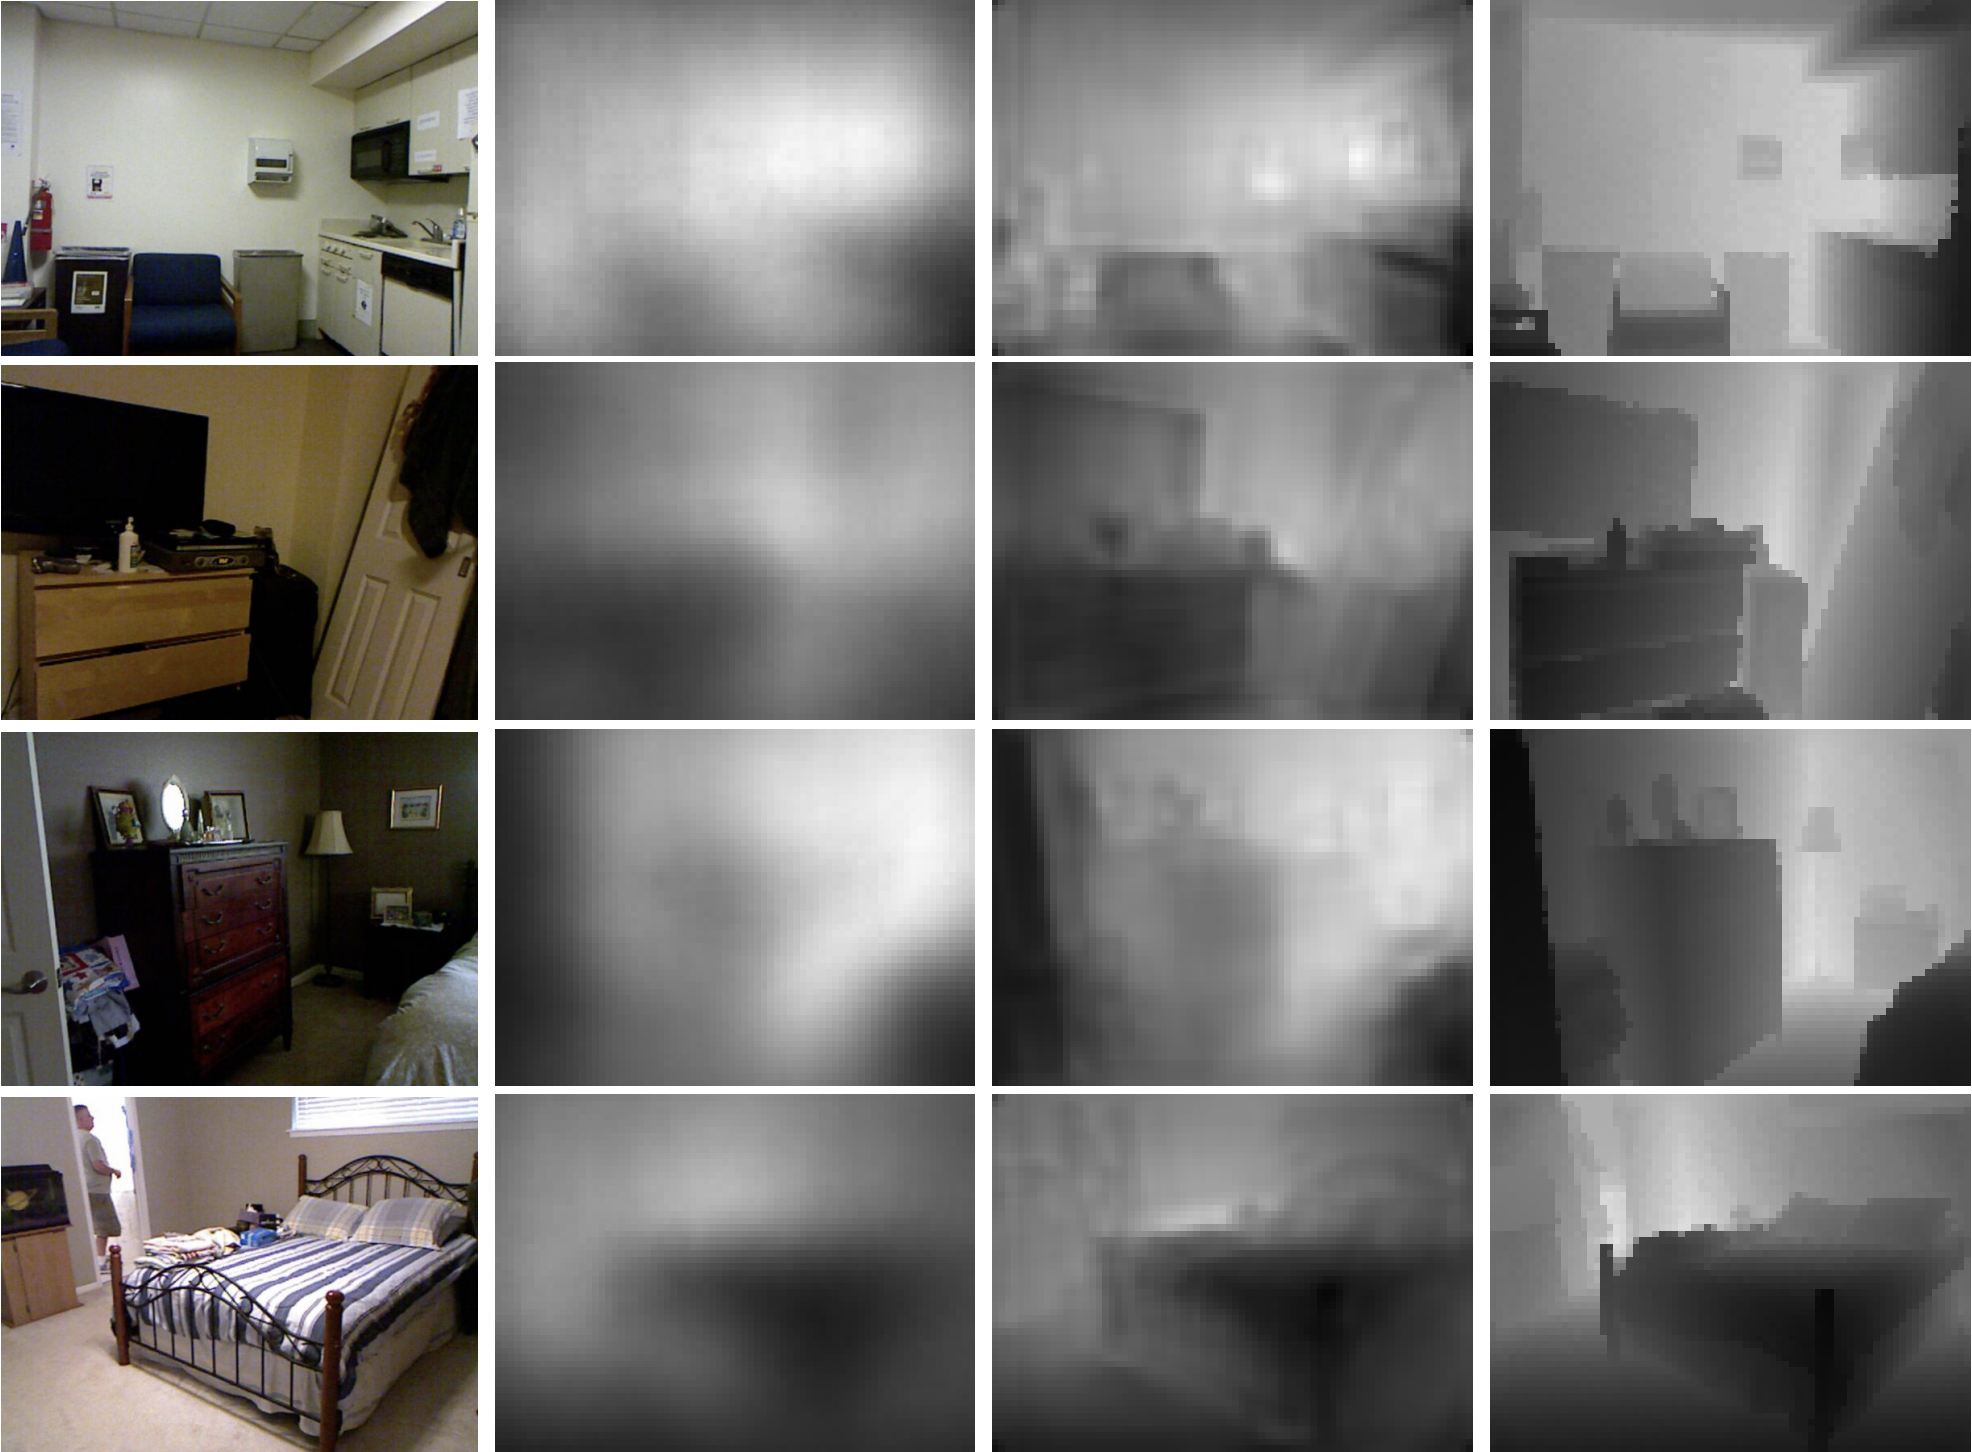
\includegraphics[width=0.8\linewidth]{Figures/SOA/ref-eigen}
	\caption[Eigen et al. Results on NYU dataset.]{Eigen et al. Results on NYU dataset. From left to right: input image, coarse estimation, refined estimation and ground truth.}
	\label{ref-eigen}
\end{figure}

This fact implies the sacrifice of the categorization of local features in favor of a learning of global features. Consequently, this part removes the invariance pose to densify the intermediate latent space.
In a second step, the scale-invariant error allows to introduce a further dimension to the learning. Rather than considering the pixel correspondence by simply using an absolute error, this function allows to partially force the depth relation between pixels. In consequence, the proposed approach is no longer considered as a classification at the pixel level but as an estimation of the depth of the image.
As shown in the Figure \ref{ref-eigen}, the results obtained are impressive and above all will set the state of the art for the field by exceeding all previous performances regardless of the outdoor or indoor environment.


Following this major contribution, this first method has been improved. In 2015, Eigen and Fergus \cite{eigen2015predicting} added the semantic and normals to surface estimation by improving the previous method. Then, using multi-scale approach and by modifying the previous loss, they were able to improve the initial approach. Indeed, while adding a segmentation capability of estimation exceeding previous works, they also were capable to improve their previous outstanding performance.

Next, following these approaches, a multitude of contributions emerged. Liu et al. \cite{liu2015deep} proposed to investigate a joint collaboration between DCNN and continuous conditional random fields (CRF) showing great performance while having an unsmooth patch-like estimation due to super-pixel pre-segmentation for neighborhood relationship modeling.
Another approach is Roy and Todorovic's \cite{roy2016monocular} proposing CNN embedded neural regression tree enforcing the smoothness of output. 
 
\cite{xu2017multi} investigate even more on CRF by introducing a multi-scale dimension to the estimation. Therefore, they created dedicated C-MF blocks which allows multi-scale fusion through the whole process. In consequence, this contribution proved an extensive performance exceeding all the previously cited works.

In addition, as an one-of-a-king approach, \cite{cao2017estimating} proposed to formulate the problem of depth estimation as a pixel-wise classification (can be assimilated as PwSS) problem. Indeed, they suggested the learning task is easier as formulated. As a finality, a CRF is applied to refine the map through local coherency reinforcement.

To cite a few other semi-supervised approaches, \cite{guo2018learning,kundu2018adadepth,fu2018deep,klodt2018supervising}, have all contributed to the growth of the field. 
Whether using a stereovision-based approach, adversarial learning, an ordinal regression formulation or a supervised SfM pre-computation, these methods require at least an intermediate depth estimation step. 

A trend can be observed in the evolution of the field of (semi-)supervised depth estimation. Over the years, the algorithms have benefited from hardware support which has made it possible to evaluate such algorithms, despite their increasing complexity. In contrast, in addition to this prevailing tendency, each of these methods shares a common disadvantage. Indeed, they require a massive amount of annotated data and moreover, these datasets in addition to being consequent must be representative. 
Moreover, most datasets have annotations that depend on the acquisition process. As expressed in part \ref{depth-acqu}, and to consider the example of KITTI, LiDaR is not infallible, especially in urban areas which contain many specular or refractive areas. As follows, when one supervises an algorithm with erroneous data, the model is necessarily influenced.

As a consequence, alternative self-supervised approaches have been developed to emancipate from annotation through a loss that does not require external information.

\subsubsection{Self-supervised learning}\label{usl}

Self-supervised depth estimation represent an extensively active domain in recent years. The concept comes from an observation concerning prior methods: the necessity of a ground truth is extremely restrictive. As mentioned before, in some cases the targets are unreliable enough and their acquisition is expensive.
This field has even metamorphosed from another estimation method to the desire to create labels. In this manner, the ambition of this kind of algorithm is to equal or even surpass the performance of sensors allowing a direct acquisition of this physical information that is the sensor-object distance.
The primary concept is based on the same principles as standard self-supervised learning, i.e. a generalizing, discriminating and differentiating cost function, but also on the necessity of ground truth only for quantitative evaluation. Hence, the algorithms are independent and can exclusively refer to the information they receive or produce to deduce the result by optimizing the loss function.

Fundamentally, the cost functions are similar across algorithms. They predominantly consist of the assembly of several terms of which two are extensively present: the reconstruction term and the smoothing term.

In this section, we will address two diverse types of algorithms: self-supervised stereo-based supervision and self-supervised monocular-based supervision. In the repertoire presented here, we will consider that the method is considered monocular if its inference is made monocularly. Consequently, some algorithms requiring two views for the learning period will remain valid for our selection criteria. 
In addition, a quantitative evaluation sub-part will display the different algorithm performances on the KITTI dataset's eigen split. This benchmark remain the reference in the domain as well as being freely available since it represents the comparison sample for the community.
Last, the last sub-part will summarize and draw conclusions on the field to position the contributions of this manuscript in this research landscape.

\textbf{Self-supervised stereo-based. } This subpart of monocular depth estimation relies on a key point which is the training with a stereo image pair. These approaches are almost all based on the principles mentioned in section 1, with the difference that the processing core is a DL network and that consequently the loss and the images are sized for this computing node. 


In 2016, Garg et al.\cite{garg2016unsupervised} proposed an image reconstruction loss-based training procedure to infer depth. Founded on an auto-encoder architecture, their approach predict an inverse-depth image which then derive an inverse warp allowing a photometric error between this synthesized image and the primary one.
\begin{figure}[h]
	\centering
	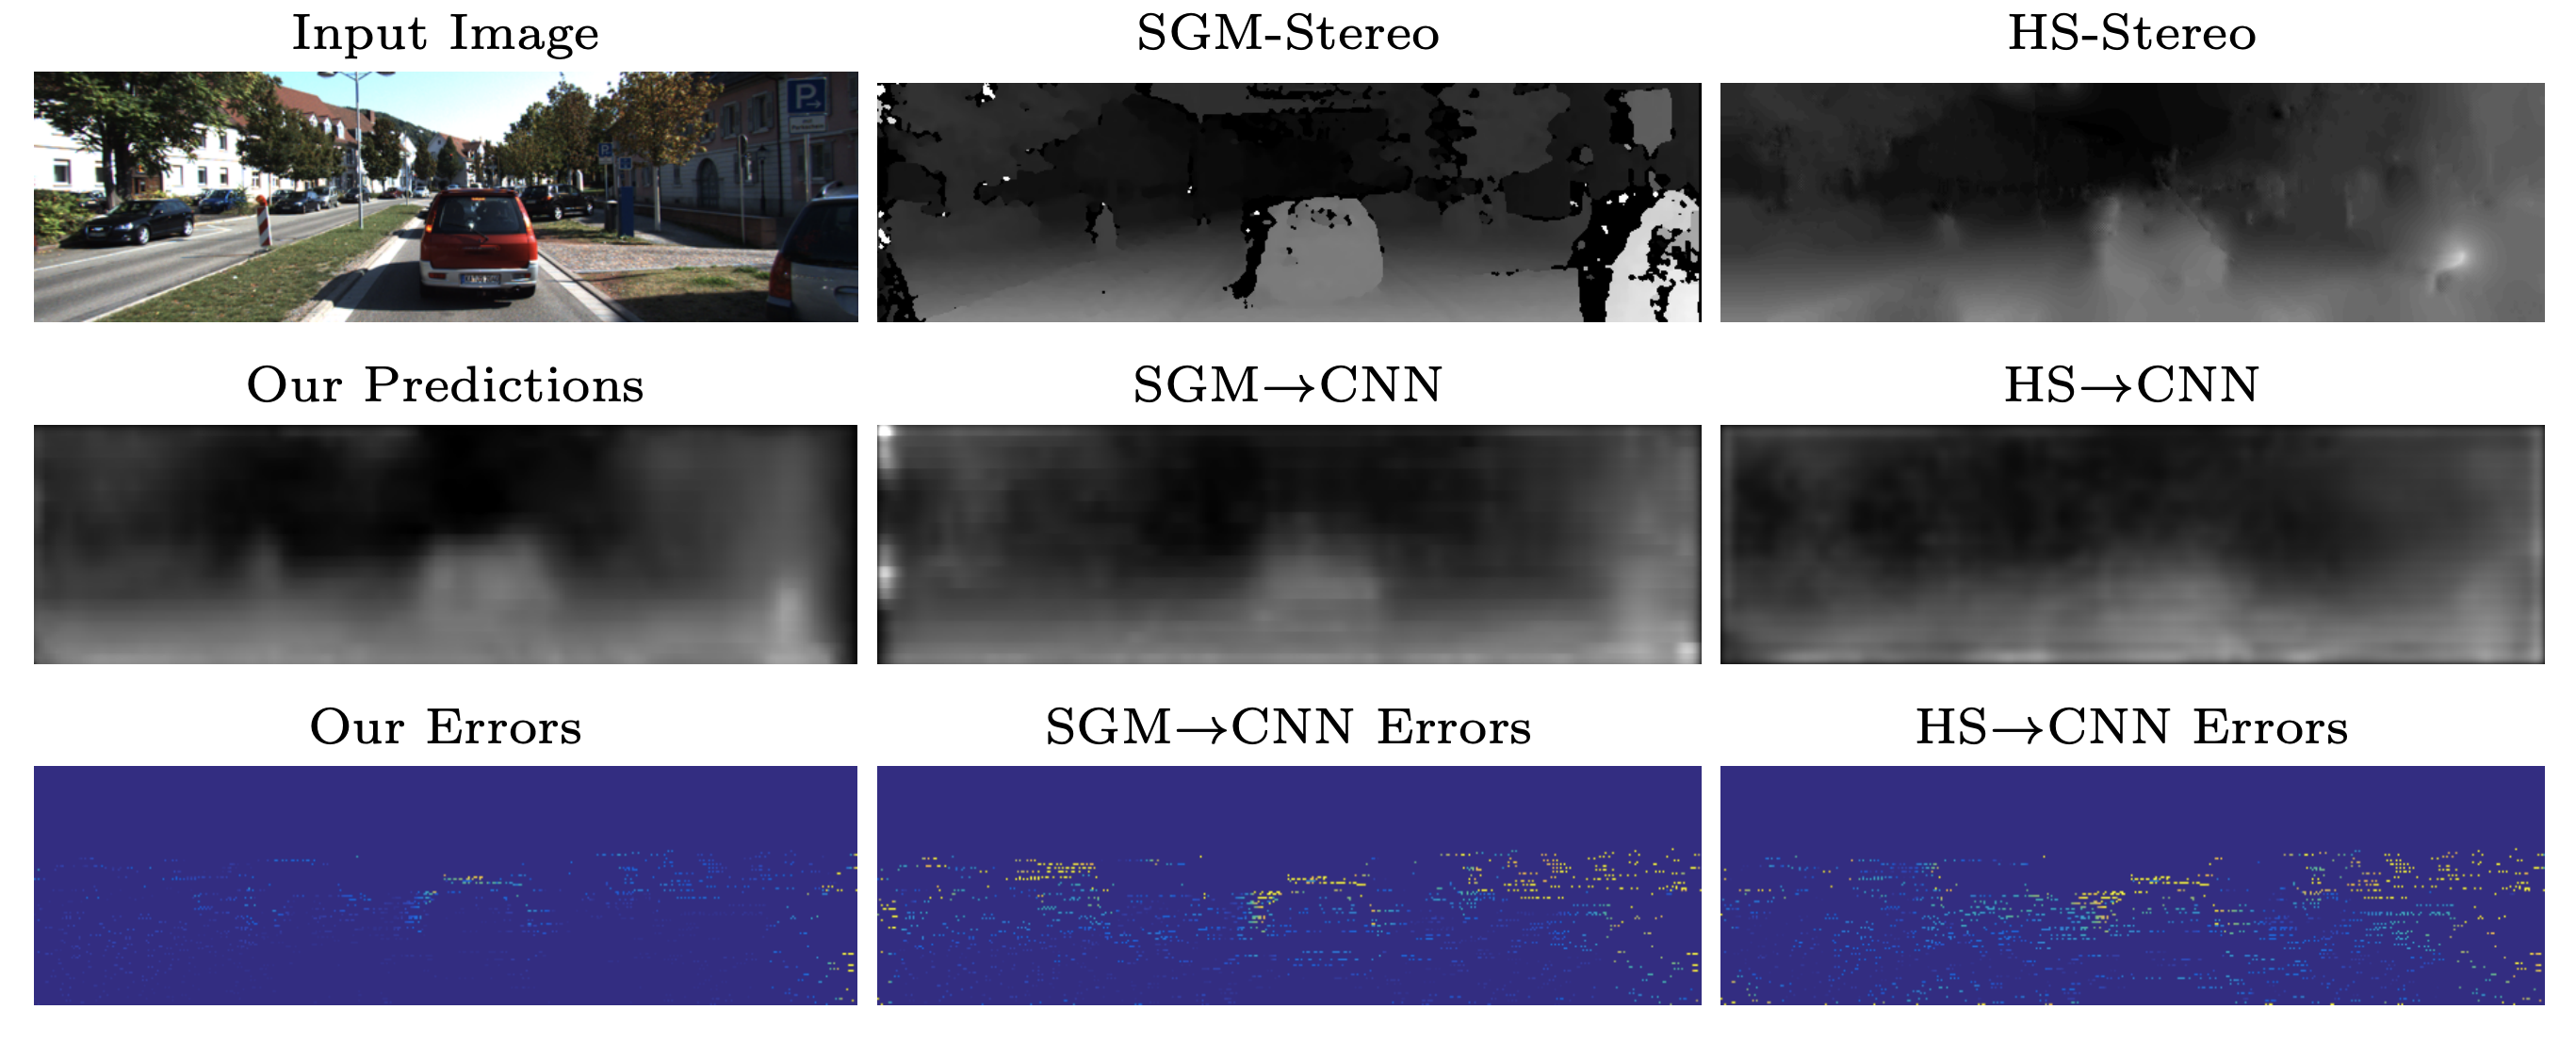
\includegraphics[width=0.8\linewidth]{Figures/SOA/illugarg}
	\caption[Results proposed by Garg et al.]{Results proposed by Garg et al. \cite{garg2016unsupervised} highlighting error reduction compared to other methods.}
	\label{illugarg}
\end{figure}


Although this pioneering approach offers advantages, their image generation-dependent minimization method is undifferentiable. Consequently, at the cost of an increased optimization complexity, they require the use of Taylor approximation to linearize their deformed image and hence, allow the computation of a gradient. As shown in Figure \ref{illugarg}, this approach displayed accurate performances explicitly comparing to direct competitors semi-global matching \cite{hirschmuller2007stereo}.


One year after, \cite{godard2017unsupervised} brings the left-right consistency concept as a term in the minimizable loss. Simplifying, the method consists in generating an opposite image. Using the spatial transformer network and its sampling blocks \cite{jaderberg2015spatial}, this consists of reformulating the perspective geometry statement by recreating a projection.

\begin{figure}[h]
	\centering
	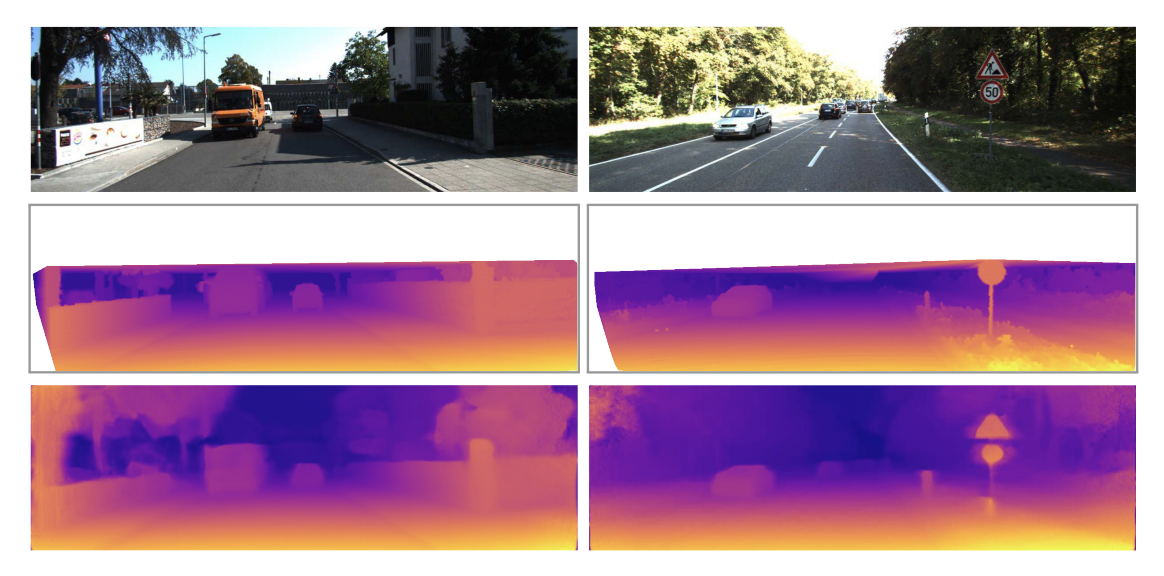
\includegraphics[width=0.8\linewidth]{Figures/SOA/illugod1}
	\caption[Godard et al. qualitative results.]{Godard et al. qualitative results.}
	\label{illugod1}
\end{figure}


Moreover, Godard et al. propose to complexify the smoothness function to include an \emph{edge-aware} effect that avoids edge blurring. For information, the smoothness term allows attenuating the discontinuity in the estimation due to the gradient of the image. This contribution proposes the addition of a third term called \emph{Left-Right Disparity Consistency Loss} ensuring equality between the first view and the second view projected with the deduced disparity. As shown in the qualitative evaluation presented in \ref{illugod1}, the predicted depth succeed into inferring depth while preserving smooth transitions along distance and salient edges.


Investigating a radically different proposal, \cite{mehta2018structured} suggests the possibility of generating depth maps using Generative \emph{Adversarial Networks} (GAN) \cite{goodfellow2014generative}. As shown in Figure \ref{illumehta}, from an input RGB image, a generator will infer a depth map which then will be discriminated.

\begin{figure}[h]
	\centering
	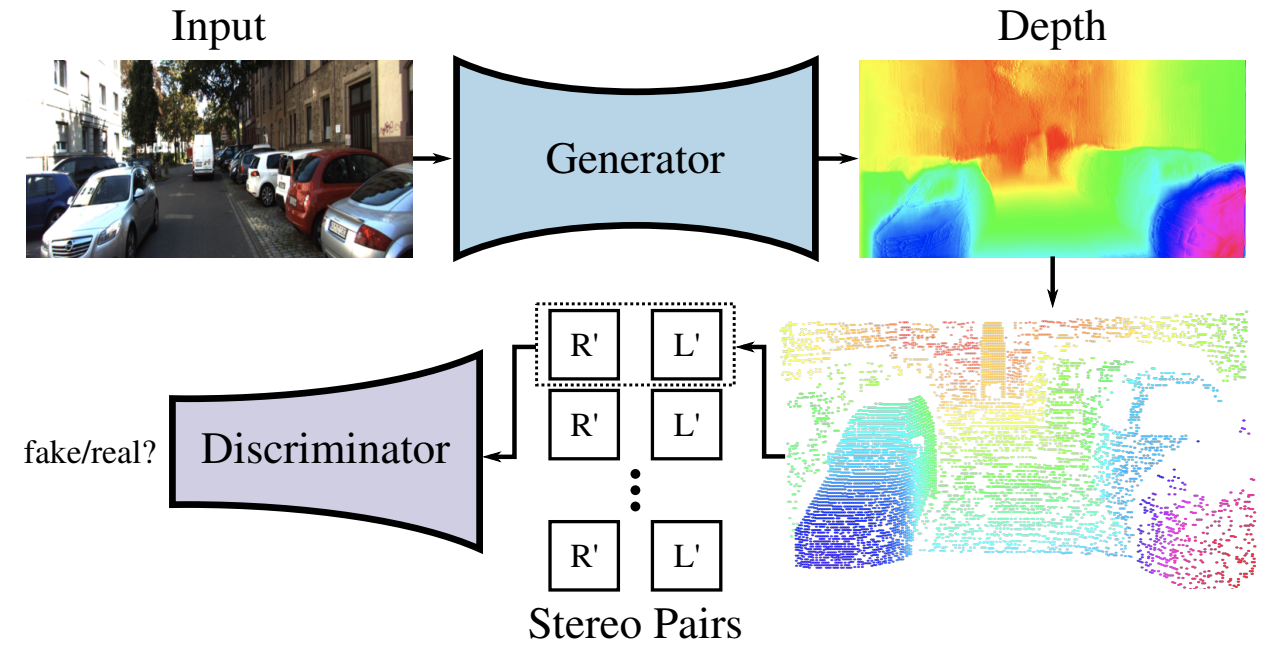
\includegraphics[width=0.8\linewidth]{Figures/SOA/illumehta}
	\caption[Mehta et al. GAN Architecture.]{Mehta et al. GAN Architecture.}
	\label{illumehta}
\end{figure}

The concept of GAN initially consists in the synthetization of photo-realistic images. Within the framework of this approach, it is a question of transposing the space of the colorimetry to the depth. Consequently, the discriminator is improved to ensure a valid estimation. To do so, the task of this network is to distinguish whether a generated view is plausible with reference to the real image collection. Once this network is valid, Mehta et al. train the generator that will produce the depth images using a camera-transformation matrix provided. Finally, the competition of these two agent networks with the help of the associated losses largely inspired by \cite{godard2017unsupervised} 
ultimately allow inferring an accurate depth map.
It is notable that usually this kind of method based on photorealism generation tends to fail when it comes to generalization. In spite of this fact, \cite{mehta2018structured} was able to show strong generalization capabilities which implicitly means that a physics norm has been infused into the network.


To complete this review of various stereo-based methods, we propose a discussion of the trinocular assumption based system from Poggi et al.\cite{poggi2018learning}. 

\begin{figure}[h]
	\centering
	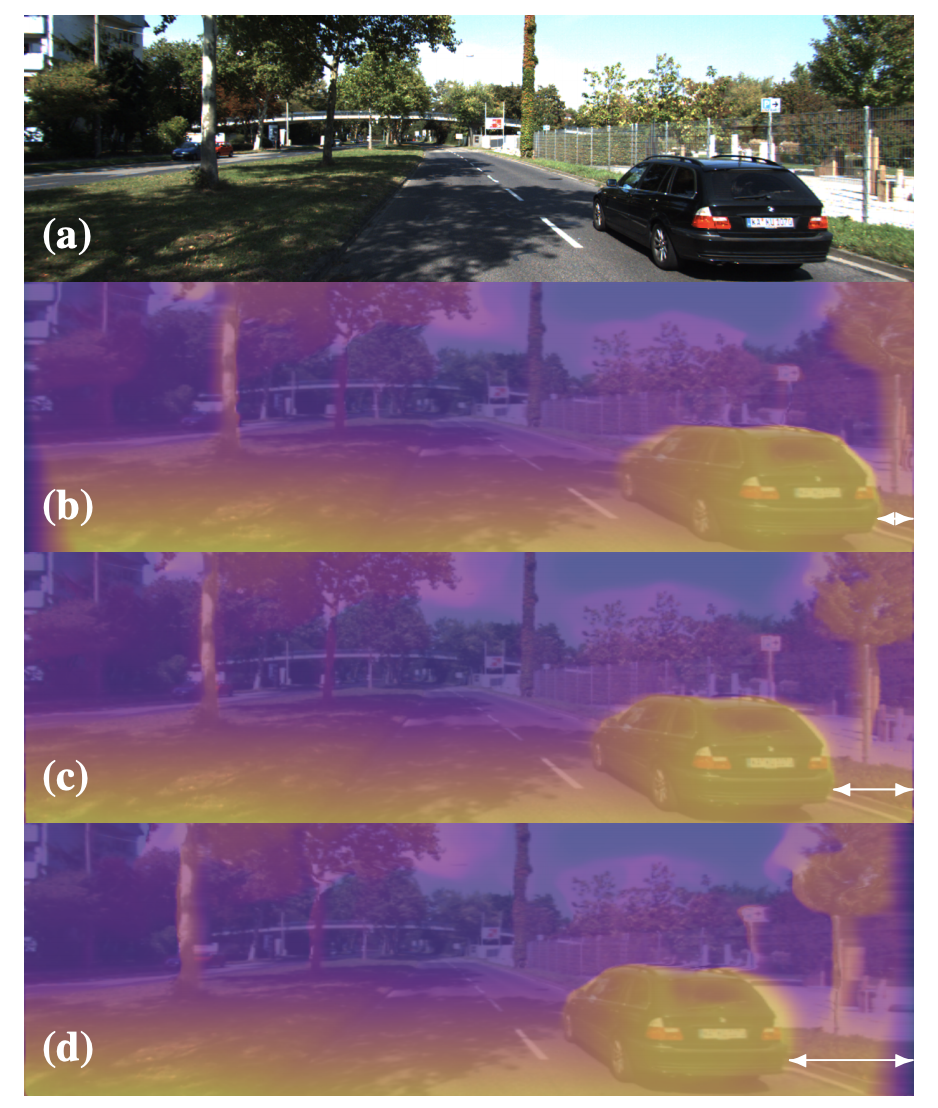
\includegraphics[width=0.5\linewidth]{Figures/SOA/illupoggi}
	\caption[Poggi et al. quanlitative evaluation.]{Poggi et al. quanlitative evaluation. a) is the input image, b) and d) are respectively the left and right estimation while c) is the center (image-aligned) estimation.}
	\label{illupoggi}
\end{figure}


This approach is mainly inspired by the different drawbacks of the previously mentioned methods. Indeed, the stereo systems suffer from the same constraints as the acquisition system. Occlusion, object boundaries and left image borders represent a significant challenge for these algorithms. Counteracting, \cite{poggi2018learning} proposes to emulate two views using the input as central image instead of one (for the stereo setup). As shown in Figure \ref{illupoggi}, the effect of such a procedure is, in addition to improving the accuracy, to eliminate the defects of the stereo system.


Many defects are present due to the use of a stereo based training procedure. Some have been reported like inconsideration of the occlusion or erroneous estimates due to second view hallucination.
In spite of this, these methods have reported results that have successively become references in the field. However, one factor remains crucial: the data. The chief drawback of such methods remains the training requirements. The use of an image pair, in addition to introducing constraints, is heavy and not necessarily available. Also, the necessary acquisition system is necessarily more constraining.
This is one of the major reasons why other methods requiring only one camera have been developed. Thus, the core concept of monocular estimation is no longer limited to the inference process but also to the training process.

\textbf{Self-supervised monocular-based. }Now that different stereo-based methods have been discussed, it is possible to shift towards monocular approaches which are nevertheless increasingly widespread.
Indeed, the fundamental interest of such an approach remains the training with a single camera. Taking advantage of the use of the temporal dimension, these techniques are based on principles similar to depth estimation by pure image processing by considering the displacement between cameras to infer a disparity. 

As a first outstanding contribution, \cite{zhou2017unsupervised} proposed to exploit the displacement between two successive images to infer depth. 

\begin{figure}[h]
	\centering
	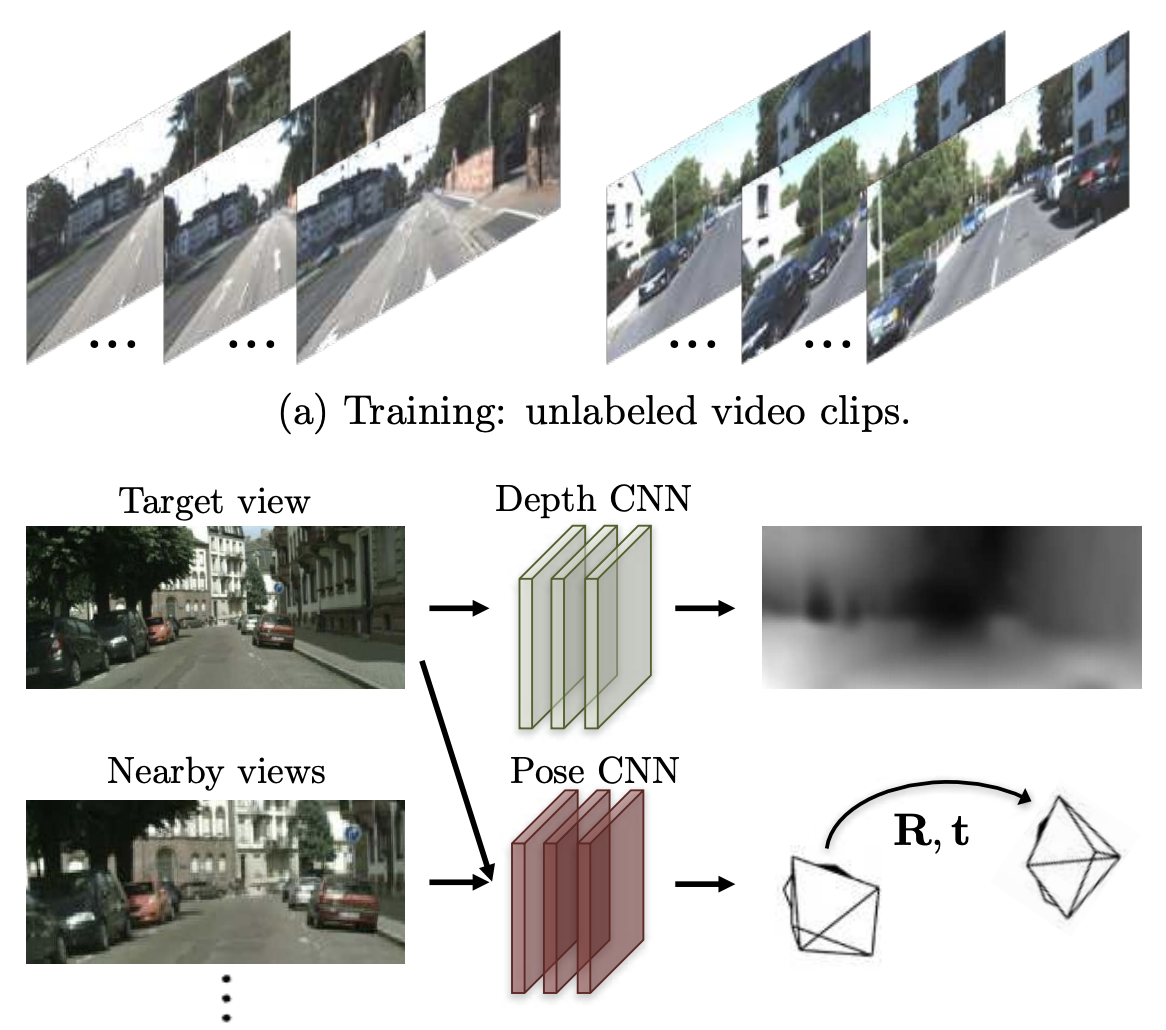
\includegraphics[width=0.5\linewidth]{Figures/SOA/illuzhou2017}
	\caption[Zhou et al. Architecture.]{Zhou et al.\cite{zhou2017unsupervised} Architecture.}
	\label{illuzhou2017}
\end{figure}

As shown in Figure \ref{illuzhou2017}, they allowed an advance towards a unified framework composed of two networks. One network estimates the depth from a first view at time $t$. A second network then tries to determine the displacement between this first view $I_t$ and a second one at time $t+1$ denoted $I_{t+1}$. Thus, similar to the no-learning-involved approach, this displacement $\{R,t\}$ allows the inverse deformation of the secondary image(s). Since a depth map and a camera pose are estimated, it is possible to project an image $I_{t+1}$ on the source view $I_{t}$. Thus, this deformation allows computing a photometric error between the projected views and the target image. Zhou et al. also emphasized some limitations of these architectures and proposed a set of overcomes. They determine a recurrent and problematic situation is the low-texture regions. Their solution is then based on approaches making the same observation (e.g. \cite{garg2016unsupervised},\cite{godard2017unsupervised}). They then propose to use an explicit multi-scale approach by forcing it directly into the network. Then, they explain in the cost function a weighted smoothing term. From these two actions, the gradient errors emanating from textureless regions are reduced and allow a perennial optimization. \cite{zhou2017unsupervised} also define a set of rules that allow the definition of operating cases.Thus, they determine that the scene must not present any moving object, not compoter any (dis)occlusion and observing only Lambertian surfaces. These three assumptions guarantee a sane gradient. 
These rules are critical since these problems will either be addressed in the next contributions described below or in the manuscript presented here.


In the same year, Yang et al. \cite{yang2017unsupervised} propose a \emph{edge-aware} approach. Contrary to a large majority of approaches, they decide to use normals which are a derivative of the depth. They claim this step allows a more geometrically faithful reconstruction. To integrate this concept, this contribution integrates layers specialized in this depth-to-normals conversion directly into the DCNN. As shown in Figure \ref{illuyang2017}, their architecture allows a bi-directional availability of the normal fields and thus to regularize with it.
This supplemental information can be derived from the depth implementing convolutions by considering the neighboring pixels.

\begin{figure}[h]
	\centering
	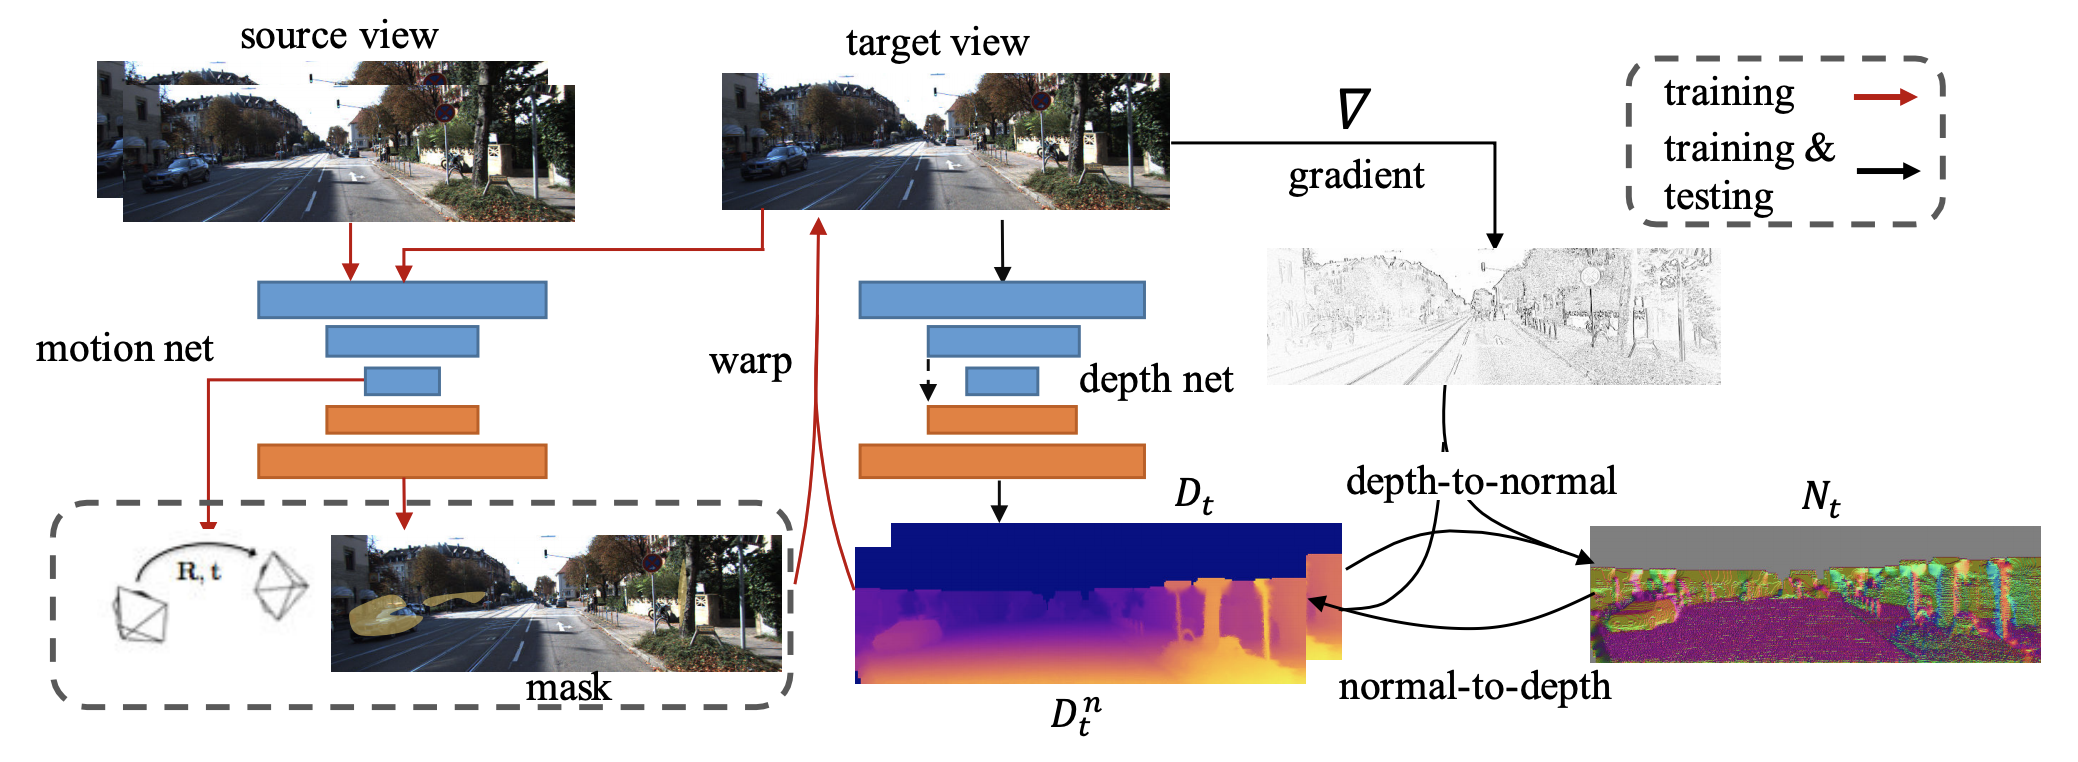
\includegraphics[width=0.8\linewidth]{Figures/SOA/illuyang2017}
	\caption[Framework propoed by Yang et al.]{Framework propoed by Yang et al.\cite{yang2017unsupervised}.}
	\label{illuyang2017}
\end{figure}


To come back briefly on the aspect \emph{edge-aware}, which constitute also a substantial part, they propose to modify the traditional smoothing function. Moreover, Yang et al. implement the use of the second order derivative allowing to eliminate ambiguities due to the surfaces but also to attempt reducing the bearing effect of the estimates.


In 2018, Mahjourian et al.\cite{mahjourian2018unsupervised} decide to focus on the geometric aspect by considering errors in 3D space. Thus, they operate a loss function composed of disciminant errors in two dimensions, 2D and 3D. 
This method also introduces a novel game-changing approach allowing to filter the areas of interest and to mask in an innovative way the out-of-bounds pixels to eliminate the remanent errors. In conclusion, their method considers a four-terms loss composed of a 3D cloud point alignment error, a 2D reconstruction error, a smoothing term and a dissimilarity measure.

\begin{figure}[h]
	\centering
	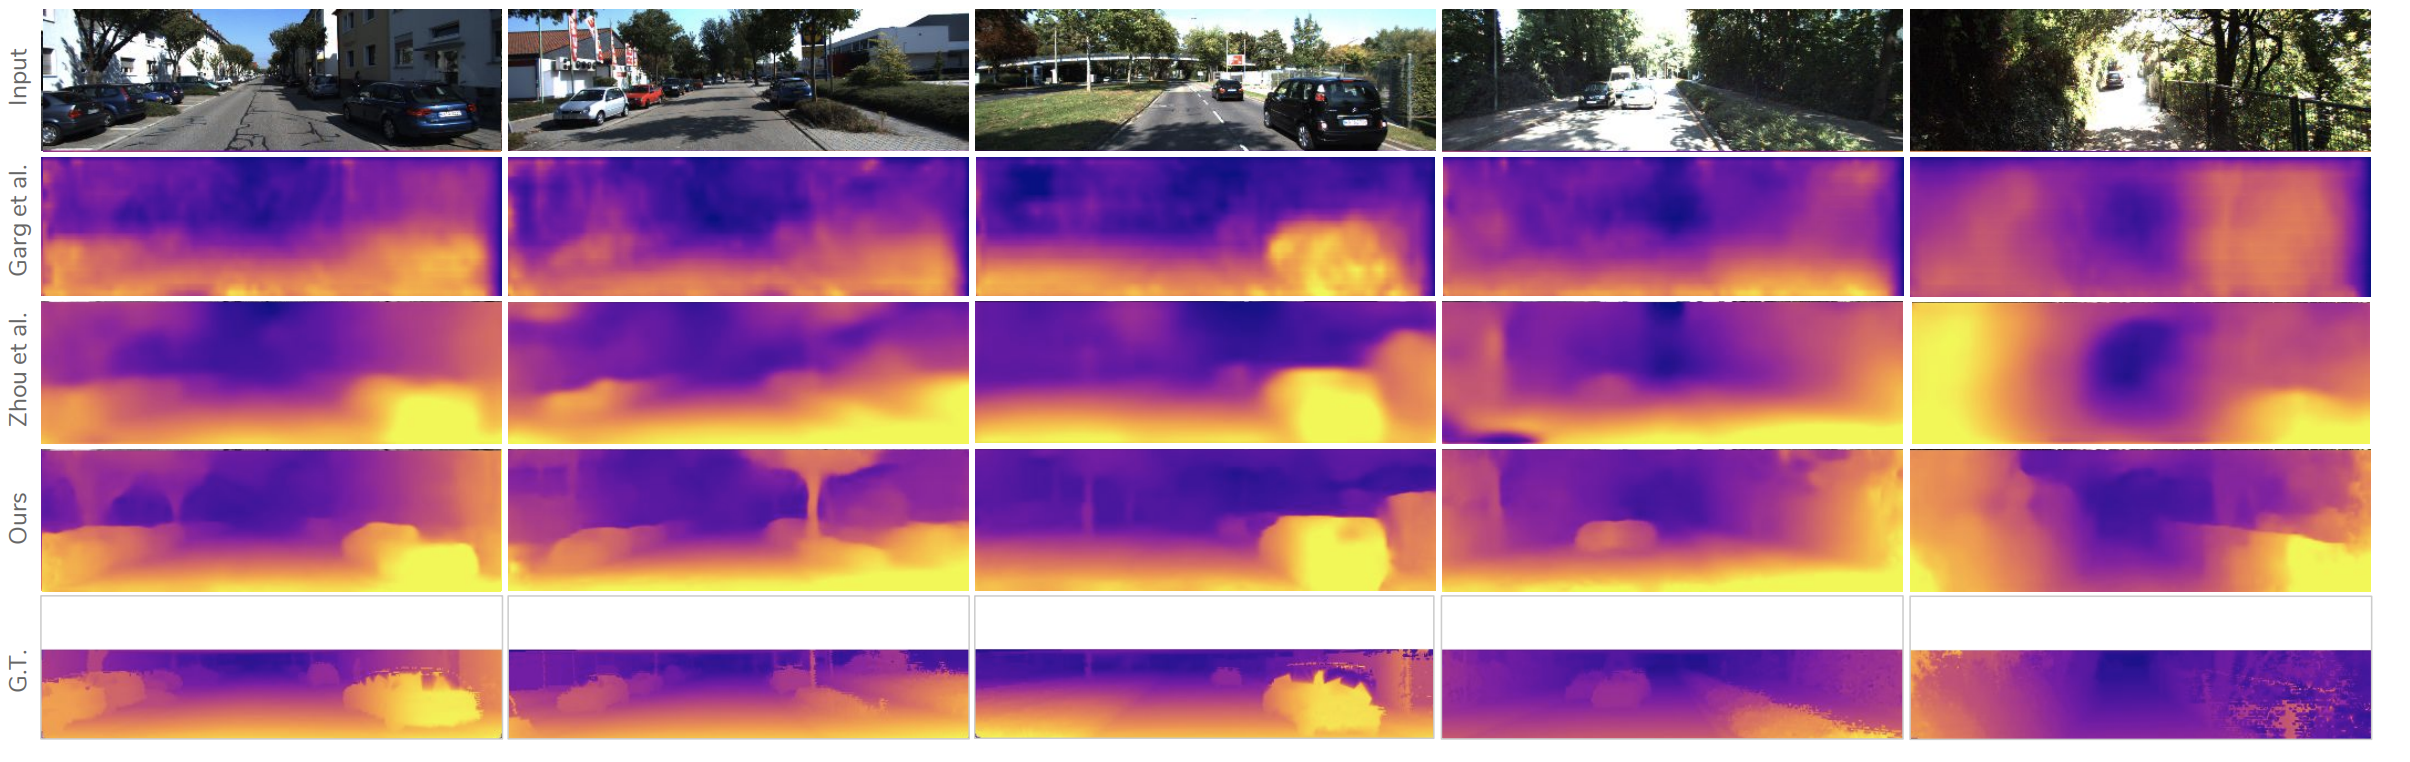
\includegraphics[width=0.8\linewidth]{Figures/SOA/mahjourian-illu}
	\caption[Mahjourian et al. Qualitative evaluation compared to previous methods..]{Mahjourian et al.\cite{mahjourian2018unsupervised} Qualitative evaluation compared to previous methods.}
	\label{mahjourian-illu}
\end{figure}


As shown in Figure \ref{mahjourian-illu}, their qualitative study highlights performance exceeding previous completions. \cite{mahjourian2018unsupervised} also demonstrates quantitatively, on the Kitti Eigen split benchmark, their performance is superior to previous approaches, despite a complexified loss.


The same year, GeoNet \cite{yin2018geonet} emerges and allows a triple estimation: the dense depth, the optical flow and the camera pose. To focus on the depth, the architecture named \emph{rigid structure reconstructor} is remarkably similar with the difference that they add a third block named \emph{non-rigid motion localizer} (see Figure \ref{geonet}).

\begin{figure}[h]
	\centering
	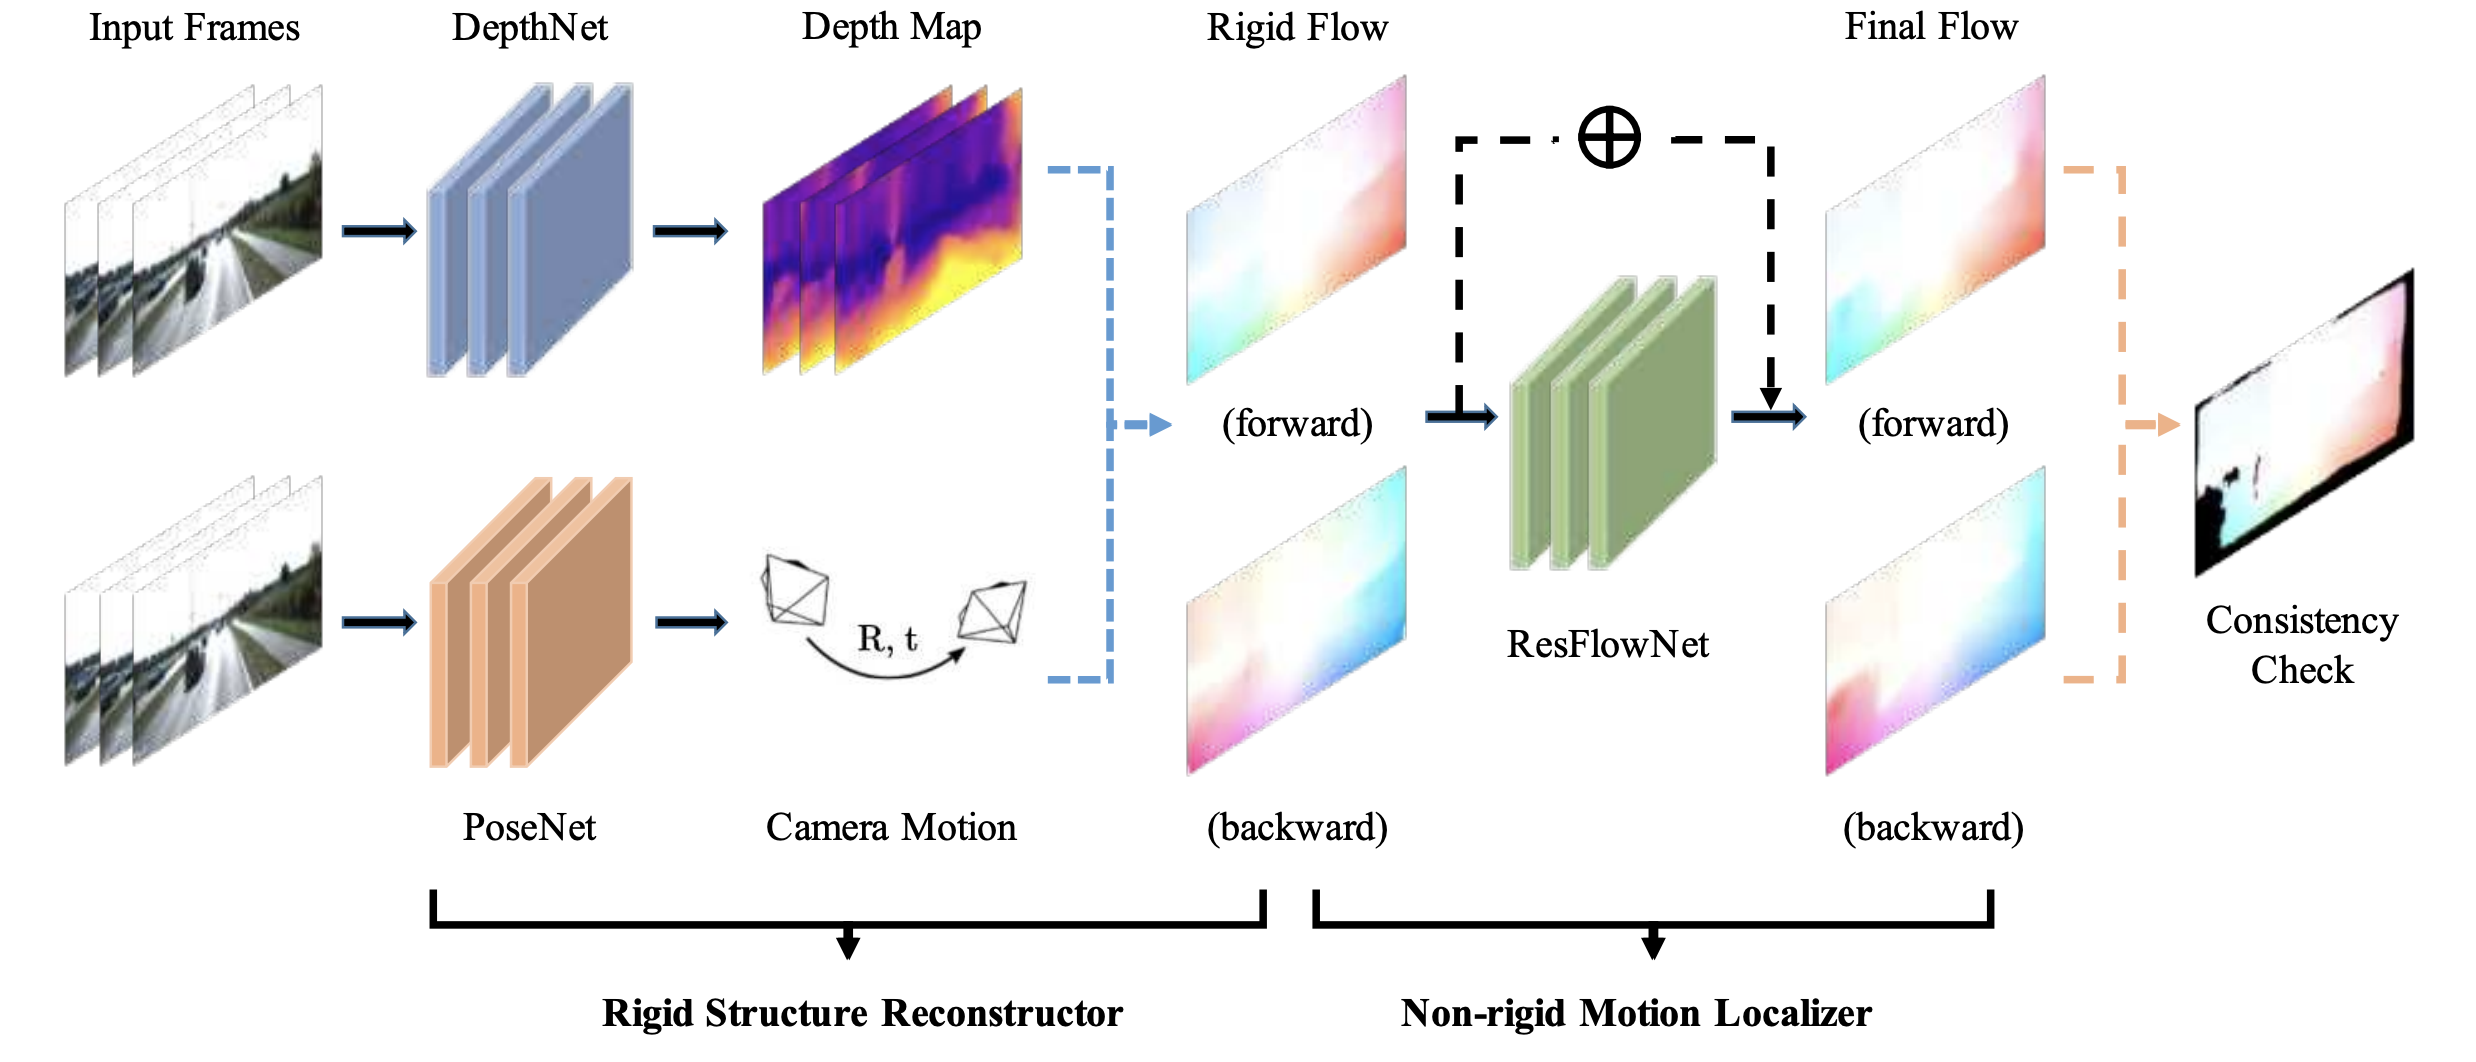
\includegraphics[width=0.8\linewidth]{Figures/SOA/geonet}
	\caption[Geonet Network.]{Geonet \cite{yin2018geonet} Network.}
	\label{geonet}
\end{figure}


Moreover, the authors attach a new importance to the choice of the loss terms and primarily consider two of the points stated by \cite{zhou2017unsupervised}. 
While their architecture \emph{rigid structure reconstructor} suffers from the same shortcomings as the previous approaches, the addition of this expansion and the associated loss allows to consider occlusion and non-Lambertian surfaces. Indeed, this part allows estimating a consistency measure which improves the robustness regarding these phenomena.


\cite{wang2018learning} proposes an originality by claiming that estimation does not necessarily require a learnable pose predictor. Indeed, this contribution proposes relying on the principles of \emph{direct visual odometry} (DVO) to eliminate this sub-architecture to estimate the displacement between two views.
Thus, the addition of a DVO \cite{steinbrucker2011real} pose predictor is used to replace the usual PoseCNN. Since it does not require training, it provides an established relationship between the estimated pose and the depth map. Moreover, this addition does not require any increased effort since it can be derived directly from the reconstructed image which equally serves as a discriminant for the DCNN. This proof of concept opened up the field of possibilities by outlining the possibility to eliminate blocks deemed essential while obtaining precise performance. 


Very similar to GeoNet\cite{yin2018geonet}, \cite{zou2018df} proposes an approach of joint estimation of depth and optical flow. The approach is slightly distinct since the architecture is drastically different. As shown in Figure \ref{illuzhou2018}, where GeoNet requires only two dissociable pipelines, DF-Net requires four. To summarize, as traditionally, a map is generated using a PoseCNN and auto-encoders allowing the evaluation of a depth consistency loss. In a second estimation pipeline, the pose estimate and the two estimated maps are aggregated to derive two maps respectively forward flow and backward flow. Ultimately, a flow is estimated from the two initial views and these same two maps can be estimated using a FlowNet. Ultimately, flow maps are deduced from the region of interest masks.

\begin{figure}[h]
	\centering
	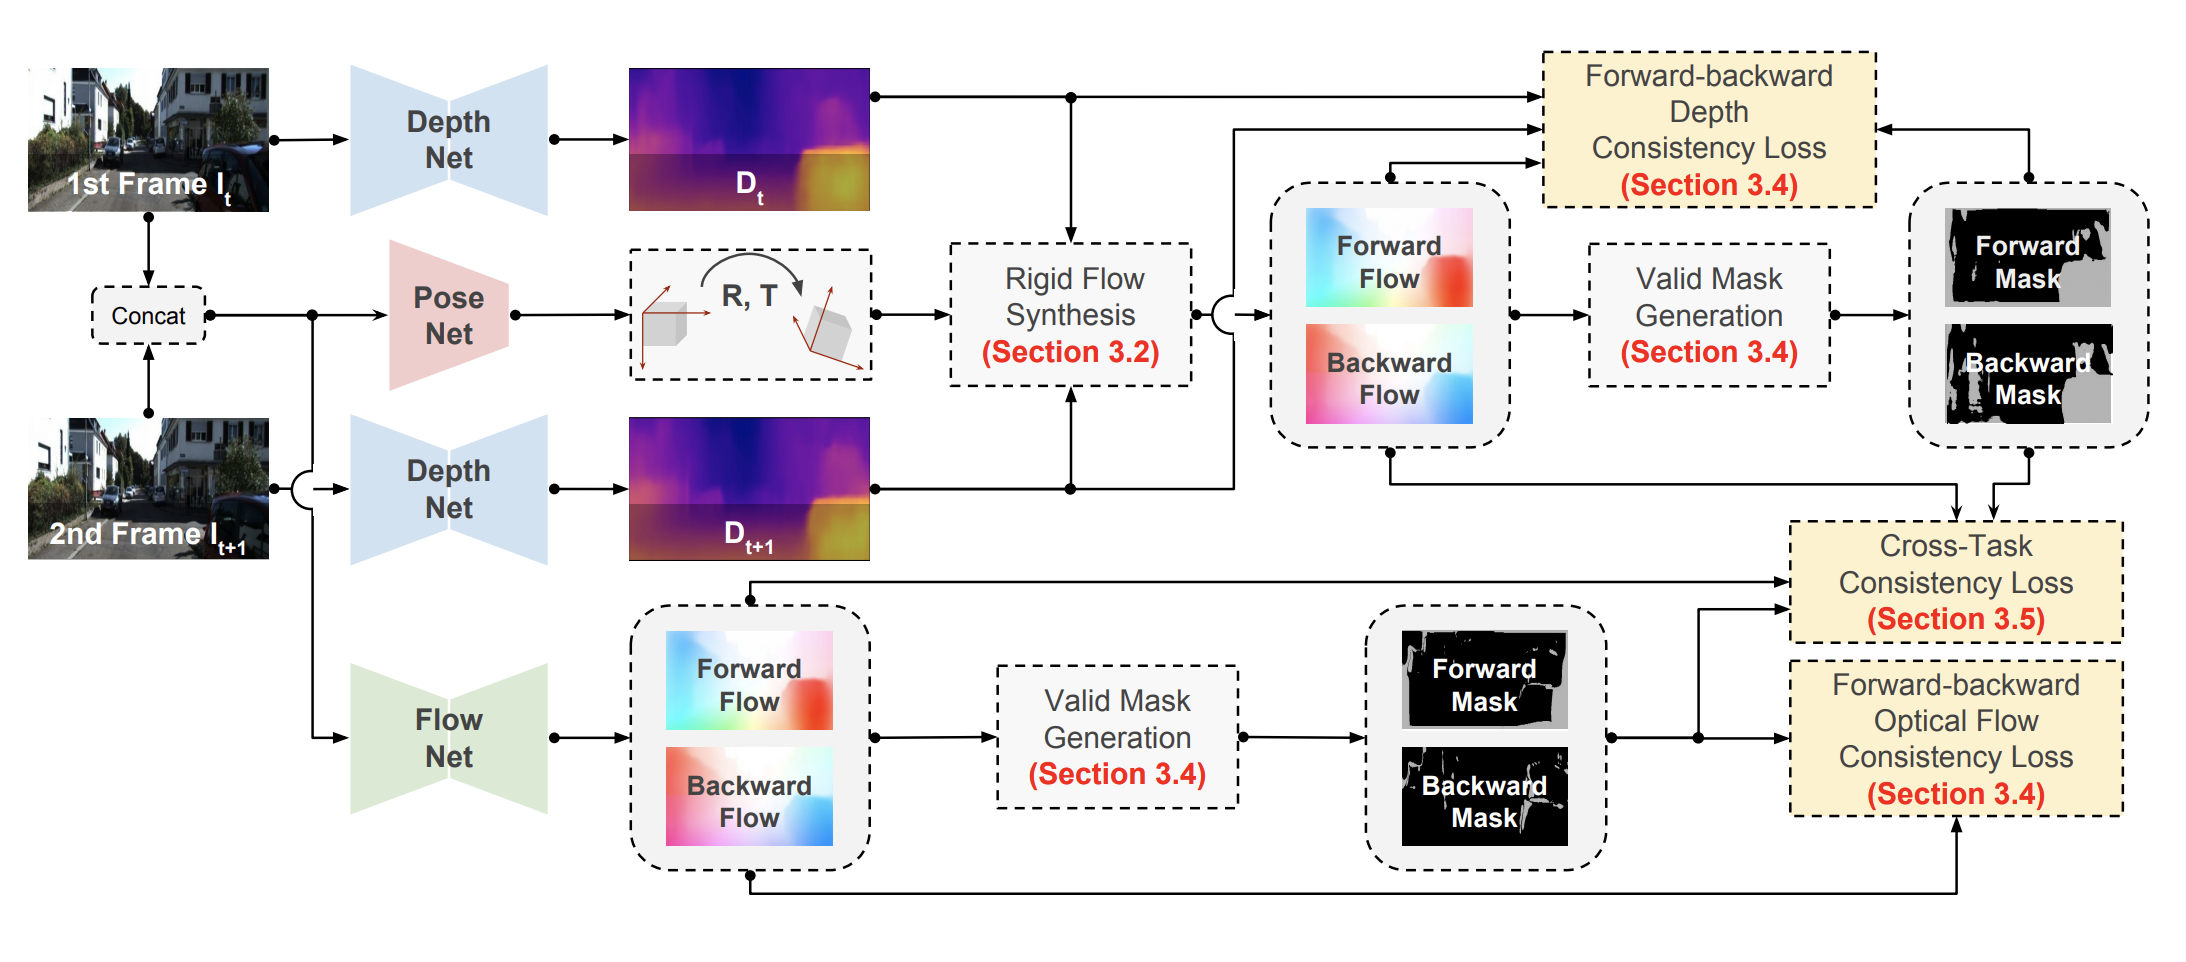
\includegraphics[width=0.8\linewidth]{Figures/SOA/illuzhou2018.png}
	\caption[DF-Net Architecture.]{DF-Net \cite{zou2018df} Architecture.}
	\label{illuzhou2018}
\end{figure}

 
All this information can be combined and compared using different terms. The \emph{Forward-backward Depth Consistency Loss} is used to ensure the consistency of forward and backward estimates. A smoothing term imposes smooth transitions while preserving the object boundaries. A photometric error is based on the assumption of brightness constancy and allows an evaluation between initial view and projection. And finally, \emph{Cross-task consistency} discriminates the differences between the optical flows estimated from the so-called rigid depth maps, and those estimated by the FlowNet. 
This method, with all the tools deployed, allows to jointly and precisely estimate a refined depth map and an optical flow. On the other hand, it is considerable the method described here represent a complicated version of GeoNet. However, the \textbf{Evaluation} sub-part will demonstrate Zou et al.'s method is slightly more efficient in estimating a depth map.


Yang et al. \cite{yang2018lego} promoted the principle of edge learning with their method called LEGO. It is based on the observation that any planar surface does not have edges until they are at the boundary of it which is similar to image processing based approaches. This allows them to define surfaces based on the absence of visual cues - here the edges -. As a consequence, it is possible to force the normals to follow the same direction for a defined surface. Based on this concept, this contribution observes a similar architecture, in two blocks, one for the depth and the other for the pose, and adds a third decoder dedicated to the edges.
Thus, employing their priors, the loss becomes a four-term minimizable function using in turn the boundary map, the depth map and the \emph{fly-out mask} allowing to eliminate the pixels not remaining in the target view due to the displacement between acquisitions. An illustration of their architecture is available below in Figure \ref{yang2018illu}.

\begin{figure}[h]
	\centering
	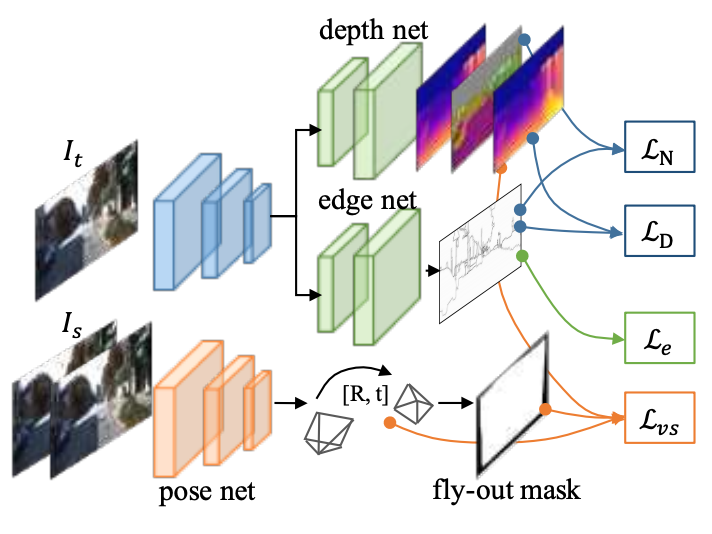
\includegraphics[width=0.4\linewidth]{Figures/SOA/yang2018illu}
	\caption[LEGO Architecture.]{LEGO Architecture \cite{yang2018lego}.}
	\label{yang2018illu}
\end{figure}


In 2019, Ranjan et al. \cite{ranjan2019competitive} propose joint learning of four descriptive images: depth, optical flow, camera motion and motion segmentation. The principal interest of this method lies in the first remarkable use of Counting Collaboration. Like so, this framework allows the joint learning of several collaborative networks in a coordinated manner. This organization is ruled by a discrimination system on the pixels according to their displacement. This core allows an explicit differentiation between moving and static surfaces deriving all previously named descriptive images in a transparent way. The authors define a training procedure including two major steps, competition and collaboration. This ultimately allows them to obtain robust results but also to generate unique descriptive images as the combination of segmented flow in the moving regions and optical flow. 


Following with another optical flow computation based approach, EPC++ \cite{luo2019every} is an extensively competitive network since it allows many current methods to compare to a very efficient network. The method starts from the fact that considering static scenes (as previously formulated) is unnecessary if we consider a network can understand the geometry of the scene as a whole. Thus, the authors propose learning jointly the 3D geometry per pixel and the motion. 

\begin{figure}[h]
	\centering
	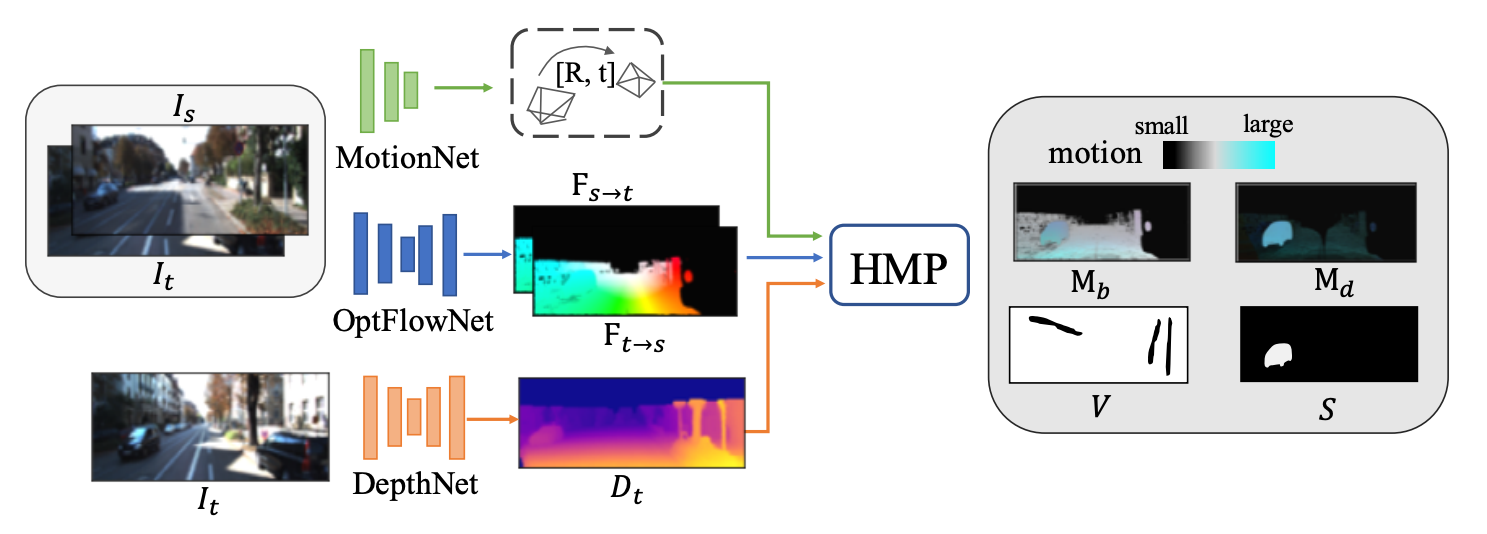
\includegraphics[width=0.8\linewidth]{Figures/SOA/illuepc++}
	\caption[EPC++ Architecture.]{EPC++ Architecture \cite{luo2019every}.}
	\label{illuepc}
\end{figure}


As shown in Figure \ref{illuepc}, this contribution opts for the use of three parallel networks each with a specific and differentiable task. A MotionNet encoder deduces the pose and two auto-encoders estimate the depth and the optical flow respectively. These three pieces of information, once given to what the authors designate an \emph{Holistic 3D Motion Parser}, allow to compute a segmentation mask for moving objects, an occlusion mask, and two 3D motion maps, one for the background, the other for the moving objects. This modeling allows to regress a precise depth map. Luo et al. also prove a network can learn to understand 3D motion at the pixel level, which emphasizes a high level of knowledge. The displayed performances show that a 3D geometry and motion concepts infused networks outperforms all previous methods.


In the same year as Luo et al. \cite{luo2019every}, Casser et al. \cite{casser2019depth} proposed a method with an original feature.This concept is based on a question: "What if 3D motion was modeled and used to refine a network on the fly? ". This method is motivated by the use of such estimators in an autonomous system. The authors subsequently propose adapting the estimation model in operation.

This contribution is based on the same setup as the significant contributions discussed above. An image sequence is used to retrieve the depth by means of the pose and deformation of consecutive images. In addition, they model a 3D motion object predictor based on the same architecture as the ego-motion predictor. Using an instance segmentation mask, Casser et al. propose to learn on-the-fly the prediction of this instance motion in 3D space. Addressing the recurrent problem of objects changing scale over time, the authors propose to allow the model to learn this phenomenon, thus avoiding the estimation errors involved. At long last, the pipeline learns on its own over time using short-training strategies on small sequences, hence reducing the discontinuity errors derived from the single-frame estimation. By this strategy, the model is refined as it observes more scenes. As shown in Figure \ref{casserillu}, this tactic allows, despite a shallower/less complex ensemble, to obtain qualitative results. Moreover, the learning complexity is reduced while making the system widely usable as an autonomous system. 

\begin{figure}[h]
	\centering
	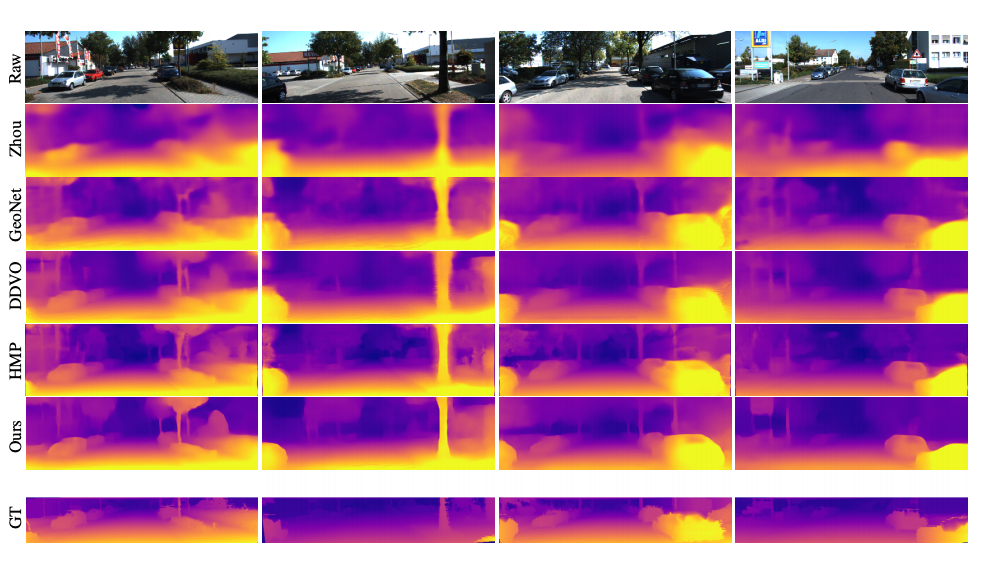
\includegraphics[width=0.8\linewidth]{Figures/SOA/casserillu}
	\caption[Quantitative evaluation of Casser et al. method.]{Quantitative evaluation of Casser et al. \cite{casser2019depth} method.}
	\label{casserillu}
\end{figure}


Neglecting this online approach, Monodepth v2 \cite{godard2019digging} is one of the best-known contributions of the community in this field. In fact, it represents, even today, the state-of-the-art in terms of robust depth map estimation. Godard et al. had in the past proposed an outstanding contribution that allowed a great advance. However, this previous method suffered from multiple flaws, one of which was the erroneous consideration of the occlusion. In reaction, the authors proposed Monodepth2, an increment of Monodepth v1.
This approach introduces three game-changer concepts:
\begin{itemize}
	\item A new design of reprojection loss to consider occlusion (\textit{Reprojection})
	\item A promising multi-scale UNet-based architecture  (\textit{Architecture})
	\item A masking strategy removing camera motion-related errors (\textit{Mask})
\end{itemize}

Embedding a dissimilarity measure and a L1 distance, the \textit{Reprojection} compare the target view with the warped second view. Although this approach is extremely similar to previouses, a \textit{Mask} is computed allowing the neglect of static pixels. As a considerable difference, while previous methods involved either optical flow or motion computation, this strategy consists solely into a per-pixel comparison of \textit{Reprojections} computed with different setups. Indeed, the \textit{Mask} is based on pixel-wise minimal photometric error between the target image and either the warped or the original second view.
Ultimately, Godard et al. proposed to benefit from UNet \cite{ronneberger2015u} skip connections as such \textit{Architecture} allow for seamless multi-scale computation. Indeed, the authors proposed to extract depth maps at intermediate layers and upsample those. Ultimately, this loss aggregation and computation at full resolution reduce texture-copy artifacts. The upsampling strategy prior to error computation enforces a correct full resolution reconstruction and avoids "holes" in the maps as usually seen in other multi-scale methods.
In Figure \ref{godardillu}, a schematic detailing the key principles is displayed.

\begin{figure}[h]
	\centering
	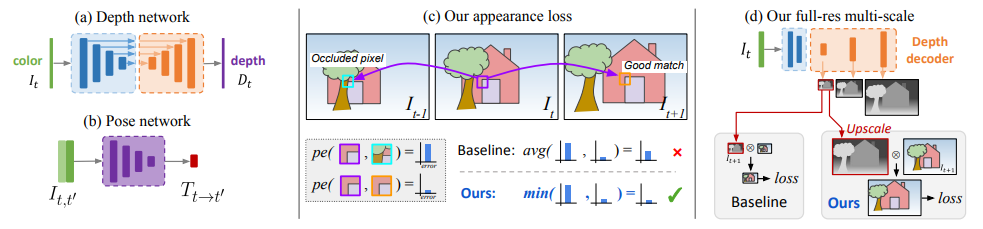
\includegraphics[width=0.8\linewidth]{Figures/SOA/godardillu}
	\caption[Monodepth v2 key principles.]{Monodepth v2 \cite{godard2019digging} key principles.}
	\label{godardillu}
\end{figure}

This approach was compared to all the methods previously explained. It clearly appears to be the most efficient, despite its reduced complexity. An absolutely remarkable fact in this contribution is the highlighting that the most important thing in a network is the objective function, especially in the self-supervised domain. Thus, a "simple" UNet can outperform other more dense methods by purely handling a properly dimensioned loss. Godard et al. have also proposed a method involving only two networks and requiring neither optical flow nor 3D motion. 
For all these reasons, this network remains the leading competitor in the race towards an accurate depth map. Therefore, this contribution will be used as a basis and benchmark for the methods developed for this manuscript. These methods will be explained in Chapter \ref{Chapter5}.



Very recently, Yang et al \cite{yang2020d3vo} proposed D3VO, an approach for joint learning of depth, pose and relative incertitude.


As improvement, some methods propose refining the depth map such as \cite{weder2020routedfusion} with RoutedFusion, or to define a depth-related uncertainty \cite{poggi2020uncertainty}.
Furthermore, some methods mobilize other further information to deduce the depth. Furthermore, many other features like semantics \cite{chen2019towards} or structured light pattern \cite{riegler2019connecting} seem to improve the estimation on an ad-hoc basis.




\textbf{Quantitative Evaluation.} This subpart proposes Table \ref{tab:evalsoadepth} to compare the different methods explained earlier. All methods have been evaluated on the Eigen Benchmark from KITTI dataset \cite{Geiger2012CVPR}.

% Please add the following required packages to your document preamble:
% \usepackage{graphicx}
\renewcommand{\arraystretch}{1.2}
\useunder{\uline}{\ul}{}
\begin{table}[h]
	\centering
	\caption[Quantitative evaluation. Comparison of depth estimation methods on KITTI 2015 the Eigen split.]{Quantitative evaluation. Comparison of depth estimation method to on KITTI 2015 \cite{Geiger2012CVPR} the Eigen split. Best results in each category are in \textbf{bold}; second best are \underline{underlined}. D is for depth supervision, D$^*$ for auxiliary depth supervision. S and M corresponds respectively to stereo and mono self-supervision.}
	\label{tab:evalsoadepth}
	\resizebox{\textwidth}{!}{%
		\begin{tabular}{lcccccccccc}
			&         &  & Abs Rel     & Sq Rel      & RMSE   & RMSE log &  & 1.25  & 1.25        & 1.25           \\ \cline{4-7} \cline{9-11} 
			Approach &
			Train &
			&
			\multicolumn{4}{c}{lower is better} &
			&
			\multicolumn{3}{c}{higher is better} \\ \hline
			Eigen \cite{eigen2014depth}                      & D       &  & 0.203       & 1.548       & 6.307  & 0.282    &  & 0.702 & 0.890       & 0.890          \\
			Liu \cite{liu2015learning}                       & D       &  & 0.201       & 1.584       & 6.471  & 0.273    &  & 0.680 & 0.898       & 0.967          \\
			Klodt \cite{klodt2018supervising}                     & D$^*$M  &  & 0.166       & 1.490       & 5.9998 & -        &  & 0.778 & 0.919       & 0.966          \\
			AdaDepth \cite{kundu2018adadepth}                  & D$^*$   &  & 0.167       & 1.257       & 5.578  & 0.237    &  & 0.771 & 0.922       & 0.971          \\
			Kuznietsov \cite{kuznietsov2017semi}                & DS      &  & 0.113       & 0.741       & 4.621  & 0.189    &  & 0.862 & 0.960       & 0.986          \\
			DVSO \cite{yang2018deep}                      & D$^*$S  &  & 0.097       & 0.734       & 4.442  & 0.187    &  & 0.888 & 0.958       & 0.980          \\
			SVSM FT \cite{luo2018single}                   & DS      &  & {\ul 0.094} & {\ul 0.626} & 4.525  & 0.177    &  & 0.891 & 0.965       & 0.984          \\
			{\underline{Guo} \cite{guo2018learning}} &
			DS &
			&
			0.096 &
			0.641 &
			{\ul 4.095} &
			{\ul 0.168} &
			{\ul } &
			{\ul 0.892} &
			{\ul 0.967} &
			{\ul 0.986} \\
			\textbf{DORN} \cite{fu2018deep} &
			D &
			&
			\textbf{0.072} &
			\textbf{0.307} &
			\textbf{2.727} &
			\textbf{0.120} &
			\textbf{} &
			\textbf{0.932} &
			\textbf{0.984} &
			\textbf{0.994} \\ \hline
			Zhou \cite{zhou2017unsupervised}                      & M       &  & 0.183       & 1.595       & 6.709  & 0.270    &  & 0.734 & 0.902       & 0.959          \\
			Yang \cite{yang2017unsupervised}                      & M       &  & 0.182       & 1.481       & 6.501  & 0.267    &  & 0.725 & 0.906       & 0.963          \\
			Mahjourian \cite{mahjourian2018unsupervised}                & M       &  & 0.163       & 1.240       & 6.220  & 0.250    &  & 0.762 & 0.916       & 0.968          \\
			GeoNet \cite{yin2018geonet}                     & M       &  & 0.149       & 1.060       & 5.567  & 0.226    &  & 0.796 & 0.935       & 0.975          \\
			DDVO \cite{wang2018learning}                      & M       &  & 0.151       & 1.257       & 5.583  & 0.228    &  & 0.810 & 0.936       & 0.974          \\
			DF-Net \cite{zou2018df}                    & M       &  & 0.150       & 1.124       & 5.507  & 0.223    &  & 0.806 & 0.933       & 0.973          \\
			LEGO \cite{yang2018lego}                      & M       &  & 0.162       & 1.352       & 6.276  & 0.252    &  & -     & -           & -              \\
			Ranjan \cite{ranjan2019competitive}                    & M       &  & 0.148       & 1.149       & 5.464  & 0.226    &  & 0.815 & 0.935       & 0.973          \\
			EPC++ \cite{luo2019every}                     & M       &  & 0.141       & 1.029       & 5.350  & 0.216    &  & 0.816 & 0.941       & 0.976          \\
			Struct2depth \cite{casser2019depth}              & M       &  & 0.141       & {\ul 1.026} & 5.291  & 0.215    &  & 0.816 & 0.945       & {\ul 0.979}    \\
			{\underline{Monodepth2 w/o pretraining} \cite{godard2019digging}} &
			M &
			&
			{\ul 0.132} &
			1.044 &
			{\ul 5.142} &
			{\ul 0.210} &
			&
			{\ul 0.845} &
			{\ul 0.948} &
			0.977 \\
			\textbf{Monodepth2 \cite{godard2019digging}} &
			M &
			&
			\textbf{0.115} &
			\textbf{0.903} &
			\textbf{4.863} &
			\textbf{0.193} &
			\textbf{} &
			\textbf{0.877} &
			\textbf{0.959} &
			\textbf{0.981} \\ \hline
			\textbf{Monodepth2 (1024 x 320) \cite{godard2019digging}} &
			M &
			&
			\textbf{0.115} &
			\textbf{0.882} &
			\textbf{4.701} &
			\textbf{0.190} &
			\textbf{} &
			\textbf{0.879} &
			\textbf{0.961} &
			\textbf{0.982} \\ \hline
			Garg \cite{garg2016unsupervised}                      & S       &  & 0.152       & 1.226       & 5.849  & 0.246    &  & 0.784 & 0.921       & 0.967          \\
			Monodepth R50 \cite{godard2017unsupervised}             & S       &  & 0.133       & 1.142       & 5.533  & 0.230    &  & 0.830 & 0.936       & 0.970          \\
			StrAT \cite{mehta2018structured}                     & S       &  & 0.128       & 1.019       & 5.403  & 0.227    &  & 0.827 & 0.935       & 0.970          \\
			3Net (R50) \cite{poggi2018learning}                & S       &  & 0.129       & 0.996       & 5.281  & 0.223    &  & 0.831 & 0.939       & 0.974          \\
			3Net (VGG) \cite{poggi2018learning}                & S       &  & 0.119       & 1.201       & 5.888  & 0.208    &  & 0.844 & 0.941       & \textbf{0.978} \\
			{\underline{SuperDepth (1024 x 382)} \cite{pillai2019superdepth}} &
			S &
			&
			{\ul 0.112} &
			{\ul 0.875} &
			\textbf{4.958} &
			\textbf{0.207} &
			&
			{\ul 0.852} &
			{\ul 0.947} &
			{\ul 0.977} \\
			Monodepth2 w/o pretraining \cite{godard2019digging}& S       &  & 0.130       & 1.144       & 5.485  & 0.232    &  & 0.831 & 0.932       & 0.968          \\
			\textbf{Monodepth2} \cite{godard2019digging} &
			S &
			&
			\textbf{0.109} &
			\textbf{0.873} &
			{\ul 4.960} &
			{\ul 0.209} &
			&
			\textbf{0.864} &
			\textbf{0.948} &
			0.975 \\ \hline
			\textbf{Monodepth2 (1024 x 320)} \cite{godard2019digging} &
			S &
			&
			\textbf{0.107} &
			\textbf{0.849} &
			\textbf{4.764} &
			\textbf{0.201} &
			\textbf{} &
			\textbf{0.874} &
			\textbf{0.953} &
			{\ul 0.977} \\ \hline
			UnDeepVO \cite{li2018undeepvo}                  & MS      &  & 0.183       & 1.730       & 6.570  & 0.268    &  & -     & -           & -              \\
			Zhan FullNYU \cite{zhan2018unsupervised}              & D$^*$MS &  & 0.135       & 1.132       & 5.585  & 0.229    &  & 0.820 & 0.933       & 0.971          \\
			EPC++ \cite{luo2019every}                     & MS      &  & 0.128       & 0.935       & 5.0111 & 0.209    &  & 0.831 & 0.945       & \textbf{0.979} \\
			Monodepth2 w/o pretraining \cite{godard2019digging} & MS      &  & 0.127       & 1.031       & 5.266  & 0.221    &  & 0.836 & 0.943       & 0.974          \\
			\underline{Monodepth2} \cite{godard2019digging}                & MS      &  & 0.106       & 0.818       & 4.750  & 0.196    &  & 0.874 & {\ul 0.957} & \textbf{0.979} \\
			D3VO uncertainty \cite{yang2020d3vo} &
			MS &
			&
			{\ul 0.101} &
			{\ul 0.772} &
			{\ul 4.532} &
			{\ul 0.190} &
			&
			{\ul 0.884} &
			0.956 &
			{\ul 0.978} \\
			D3VO ablation \cite{yang2020d3vo}             & MS      &  & 0.105       & 0.791       & 4.650  & 0.193    &  & 0.878 & {\ul 0.957} & \textbf{0.979} \\
			\textbf{D3VO full} \cite{yang2020d3vo} &
			MS &
			&
			\textbf{0.099} &
			\textbf{0.763} &
			\textbf{4.485} &
			\textbf{0.185} &
			&
			\textbf{0.885} &
			\textbf{0.958} &
			\textbf{0.979} \\ \hline
			\textbf{Monodepth2 (1024 x 320)} \cite{godard2019digging} &
			MS &
			&
			\textbf{0.106} &
			\textbf{0.806} &
			\textbf{4.630} &
			\textbf{0.193} &
			\textbf{} &
			\textbf{0.876} &
			\textbf{0.958} &
			\textbf{0.980}
		\end{tabular}%
	}
\end{table}

\textbf{Summary and conclusions. } 

As it has been demonstrated, the scientific community attaches considerable importance to depth estimation. In recent years, researchers have turned to modern deep learning methods. Indeed, this allows less constrained approaches. Regrettably, the use of these techniques ordinarily requires strong assumptions but above all a massive amount of data. Moreover, it is notable that the models trained with certain data are linked to it, and consequently, when the modality used neglects certain phenomena, so do the models. 



